\documentclass{article}
\usepackage{graphicx} % Required for inserting images
\usepackage{pdfpages}
\usepackage{geometry}
\usepackage{array}
\geometry{paperwidth=21cm, paperheight=29.7cm, top=1cm, bottom=2cm, left=2cm, right=2cm}
\usepackage{float}
\usepackage[utf8]{inputenc}
\usepackage[backend=biber,style=ieee]{biblatex}
\addbibresource{bibliography.bib} % Ton fichier .bib
\title{Memoire de PFE}
\author{malak-nesrine}
\date{May 2025}
\setlength{\parindent}{2em}
\usepackage[most]{tcolorbox}

\usepackage{url}
\usepackage[colorlinks=true, linkcolor=blue, urlcolor=magenta, citecolor=blue]{hyperref}
\usepackage[T1]{fontenc}



\usepackage{subcaption}

\usepackage{setspace}





\begin{document}
\pagenumbering{gobble} 
\DeclareFieldFormat{labelnumber}{\textcolor{red}{#1}}



\newpage
\cleardoublepage

\pagenumbering{roman}% Commence la numérotation à partir de 1
    % Redémarre le compteur de pages

% === Page des remerciements (pas de numéro visible, mais comptée) ===
\thispagestyle{empty}


\begin{center}
{\Huge \textbf{\textit{Remerciements}}}

\vspace{2cm} 
\fontsize{14pt}{16pt}\selectfont\textit{Tout d’abord, nous exprimons notre profonde gratitude envers \textbf{ALLAH}, le Tout-Puissant, de nous avoir donné la santé, la force, la patience et la capacité de mener à bien ce travail.
}

\vspace{1cm}
\fontsize{14pt}{16pt}\selectfont\textit{Nous tenons à remercier les membres du jury pour leur présence, pour la lecture attentive de ce mémoire, ainsi que pour les remarques qu’ils nous adresseront lors de notre soutenance afin d’enrichir et d’améliorer notre travail.}

\vspace{1cm}
\fontsize{14pt}{16pt}\selectfont\textit{Nous tenons à exprimer notre sincère gratitude à notre promotrice universitaire, Madame \textbf{Bensaou Nacera}, pour son soutien indéfectible, ses conseils avisés et son accompagnement précieux dès le moment où elle a fait notre connaissance. Son engagement et sa disponibilité ont été essentiels à la bonne réalisation de ce projet, et nous lui sommes profondément reconnaissantes pour le temps et l’énergie qu’elle nous a consacrés.} 

\vspace{1cm}
\fontsize{14pt}{16pt}\selectfont\textit{Nous tenons également à remercier vivement notre encadreur de l’entreprise, Monsieur \textbf{ Mohammed Chafik Baazouzi}, pour sa totale disponibilité et pour tout ce qu’il nous a apporté comme aide, connaissances et conseils, et aussi pour l'intérêt constant qu'il nous a montré tout au long de ce travail. Nous tenons à le remercier chaleureusement pour le temps précieux qu'il nous a accordé.}

\vspace{1cm}

\fontsize{14pt}{16pt}\selectfont\textit{Nous adressons nos sincères remerciements à l’ensemble des professeurs, ainsi qu’à toutes les personnes qui, par leurs paroles, leurs écrits, leurs conseils et leurs critiques, ont guidé nos réflexions, accepté de nous rencontrer et répondu à nos questions tout au long de nos recherches.}

\vspace{1cm}

\fontsize{14pt}{16pt}\selectfont\textit{%
Nos plus vifs remerciements vont également au Directeur Général, et à l’ensemble du personnel de \textbf{Gulf Insurance Group – Algérie (GIG Algéria)}, et en particulier au département informatique, qui ont mis à notre disposition les moyens les plus favorables à la réussite de ce travail.%
}



\end{center}

\newpage
\cleardoublepage
\thispagestyle{empty}

\begin{center}
{\Huge \textbf{\textit{Dédicace}}}

\vspace{2cm}

\fontsize{14pt}{16pt}\selectfont\textit{Un grand merci à nos mères et pères pour leur amour, leurs conseils ainsi que leur soutien inconditionnel, tant moral qu’économique, qui nous a permis de réaliser les études que nous souhaitions et, par conséquent, d’accomplir ce mémoire.}

\vspace{1cm}

\fontsize{14pt}{16pt}\selectfont\textit{Nous remercions sincèrement nos amis et collègues pour leur soutien et leurs encouragements tout au long de ce travail.}

\vspace{1cm}

\fontsize{14pt}{16pt}\selectfont\textit{Enfin, un grand merci à toutes celles et tous ceux qui nous ont aidés à franchir cette étape importante de notre vie. }

\end{center}

\newpage
\begin{center}
{\Huge \textbf{Table des matières}}
\end{center}
\renewcommand{\contentsname}{}
\tableofcontents
\newpage
\begin{center}
{\Huge \textbf{Liste des figures}}
\end{center}
\renewcommand{\listfigurename}{}
\listoffigures
\newpage
\pagenumbering{arabic}
\setcounter{page}{1}

% Sections et sous-sections
\section{Introduction générale}
\begin{spacing}{1.3}
\vspace{1cm}
\hspace*{2em}Dans un monde professionnel en constante évolution, caractérisé par des innovations technologiques et des changements dans les modes de communication, les compétences deviennent rapidement obsolètes. Dans ce contexte, pour les entreprises, la mise en place de formations flexibles et efficaces pour leurs employés est un enjeu stratégique majeur afin d’accompagner ces changements. Il est impératif qu'elles s'engagent à investir dans les compétences afin de maintenir leur compétitivité, leur capacité d'innovation et leur pérennité.

\vspace{1cm}

Afin de répondre à ces enjeux, les entreprises adoptent des stratégies diverses pour la formation de leur personnel. Certaines restent attachées aux méthodes traditionnelles, ne proposant que des formations en présentiel sans intégrer l’e-learning, tandis que d’autres ont adopté ce dernier à travers des plateformes externes comme Google Meet ou LinkedIn Learning, tout en maintenant des sessions en présentiel.
Cependant, ces méthodes et plateformes ne répondent pas toujours pleinement aux exigences spécifiques des entreprises, notamment en matière de réduction des coûts et de personnalisation. En outre, des insuffisances persistent dans la gestion des formations, qu’elles soient en ligne, en présentiel ou liées aux ressources pédagogiques, ce qui entrave la performance des entreprises et leur capacité à s’adapter aux évolutions rapides du marché professionnel.




\vspace{1cm}






Ces limitations ont conduit de nombreuses entreprises à aujourd’hui entamer une transition vers des solutions internes, avec des plateformes d’apprentissage privées et centralisées, leur permettant de lancer leurs propres conférences et formations, tout en conservant un contrôle total sur le processus.




\vspace{1cm}

En ce sens, notre projet de cycle a pour but de créer une plateforme, nommée TAKWINI, dédiée à la gestion de l'apprentissage pour l'entreprise Gulf Insurance Group Algeria. Il s'agit d'une solution complètement sécurisée, privée et sur mesure, réservée aux personnels autorisés. Cette plateforme mettra à disposition des ressources humaines les outils requis pour gérer efficacement les formations, depuis la réception des demandes jusqu'à la planification des sessions, tout en offrant un espace pédagogique que les formateurs pourront contrôler.


\vspace{1cm}

Ce mémoire décrit la méthode utilisée pour créer cette plateforme, les choix technologiques effectués et les résultats obtenus. Il est divisé en plusieurs chapitres organisés comme suit :

\vspace{0,4cm}

\noindent \textbf{L’analyse de l’existant :} Ce chapitre aborde l'organisme Gulf Insurance Group Algeria en analysant sa situation actuelle concernant la gestion de la formation, tout en évaluant les solutions disponibles sur le marché pour en déceler les limites et proposer une solution mieux adaptée aux besoins spécifiques de l'entreprise.

\noindent \textbf{La conception :} Nous présentons les fonctionnalités principales de notre plateforme et présentons la conception UML à travers l’ensemble des diagrammes nécessaires. Nous y exposons également le design apporté à l’interface utilisateur.

\noindent \textbf{La réalisation :} Nous déterminons les méthodes et l’architecture adoptées ainsi que les outils utilisés, et présentons également l’interface finale.








\end{spacing}



\newpage

\section{Étude de l’existant}
\subsection{Présentation de l’entreprise Gulf Insurance Group (GIG) algeria}

\vspace{0,5cm}
\hspace*{1em}Gulf Insurance Group Algeria est une société privée qui se concentre sur les assurances, en particulier pour les dommages liés aux véhicules, à l'habitation, ainsi qu'aux professionnels etc, Elle a pour objectif de satisfaire les besoins des particuliers et des entreprises en Algéria. Les membres du Gulf Insurance Group (GIG) bénéficient de l'expertise des principaux acteurs régionaux présents dans plus de 12 pays au Moyen-Orient et en Afrique du Nord. En outre, GIG Algérie possède un réseau de plus de 200 agences à travers le pays, assurant ainsi une proximité constante avec sa clientèle et un accès facilité à ses services. \cite{GIG}

\vspace{0,3cm}


GIG Algeria, en pleine transition numérique, souhaite moderniser et informatiser la gestion de ses formations, afin de faciliter et améliorer les méthodes d’apprentissage en son sein.
 C'est cette situation qui a motivé le choix de ce sujet de mémoire pour mettre en place une solution de gestion des formations.


\subsection{Analyse de la situation actuelle}
\subsubsection{Situation Actuelle}

\vspace{0,3cm}
\hspace*{1em}L’entreprise GIG Algeria est composée de 14 départements, parmi lesquels : Ressources Humaines (RH), Informatique (IT), Marketing, Comptabilité, etc...

\vspace{0,3cm}
\noindent Actuellement, l’entreprise organise régulièrement des formations pour ses employés. Ces formations peuvent être :
\begin{itemize}
    \item En ligne ou en présentiel,
    \item Internes (dispensées par les employés eux-mêmes) ou externes (dispensées par des organismes extérieurs).
\end{itemize}
\vspace{0,3cm}
L’organisation de ces formations est assurée par le service des Ressources Humaines (RH).
Les formations internes sont animées par des formateurs internes (également appelés "professeurs"). Ce sont des employés ordinaires, mais disposant des compétences nécessaires pour partager leurs connaissances à travers des cours ou des conférences. Ces formations permettent aux employés de rester à jour avec les nouvelles technologies, les menaces émergentes liées à la digitalisation, et de maintenir un haut niveau de professionnalisme.

\vspace{0,3cm}

\noindent Processus actuel d’organisation d’une formation
Lorsqu’un formateur a une nouvelle information ou compétence à partager (par exemple, après avoir assisté à une formation externe), il peut décider d’organiser une session de formation interne.

\vspace{0,3cm}

\noindent Le formateur envoie un e-mail au service RH en précisant : Le nom de la formation, La date et L’heure souhaitée, Le type de formation (en ligne ou présentielle), ainsi que les départements concernés (un formateur d’IT peut, par exemple, former les équipes du Marketing sur un nouveau logiciel).

\vspace{0,3cm}
\noindent Le personnel RH consulte le calendrier \textbf{Microsoft Teams} pour vérifier la disponibilité à la date et à l’heure demandées.

\vspace{0,3cm}

\noindent Si une autre formation est déjà planifiée à ce moment-là, la demande est refusée et une proposition peut être faite par le service RH  (autre jour ou autre heure). Sinon, la demande est acceptée.La formation est ensuite programmée dans le calendrier Teams, afin qu’elle soit visible par tous les collaborateurs concernés.

\vspace{0,3cm}

\noindent Ainsi, les formations sont intégrées au planning global de l’entreprise et gérées de manière centralisée via Microsoft Teams.
\vspace{0,3cm}

\noindent Les outils utilisés pour la planification sont: 
\begin{figure}[H]
  \centering
  \begin{subfigure}[t]{0.15\textwidth}
    \centering
    
\includegraphics[width=\textwidth]{Gmail.jpg}
    \caption{Gmail}
    \label{fig:gmail}
  \end{subfigure}
  \hspace{1cm}
  \begin{subfigure}[t]{0.15\textwidth}
    \centering
    
\includegraphics[width=\textwidth]{teams.png}
    \caption{Teams}
    \label{fig:teams-sub}
  \end{subfigure}
  \caption{Interfaces de Gmail et Microsoft Teams}
  \label{fig:teams1}
\end{figure}


\hspace{1cm}

\begin{figure}[h!]
  \centering
  % \includegraphics[width=0.6\textwidth]{}
  \begin{tcolorbox}[title=Simulation d’un e-mail de demande de formation]

De : Ahmed.Benali@gig.dz \\
À : RH@gig.dz \\
Objet : Demande de planification d'une formation – Nouvel outil CRM

Bonjour,

Je souhaite organiser une session de formation interne intitulée : "Découverte du nouvel outil CRM".

Date proposée : 20 mai 2025 

Heure : 10h00 – 11h30  

Type : En présentiel  

Départements concernés : Marketing 

Merci de me confirmer la disponibilité du créneau.

\vspace{0,3cm}

Cordialement,  

Ahmed Benali – Département IT
\end{tcolorbox}
  \caption{Structure actuelle d'un email}
  \label{fig:teams2}
\end{figure}

\hspace*{1,5em}
\begin{figure}[h!]
  \centering
  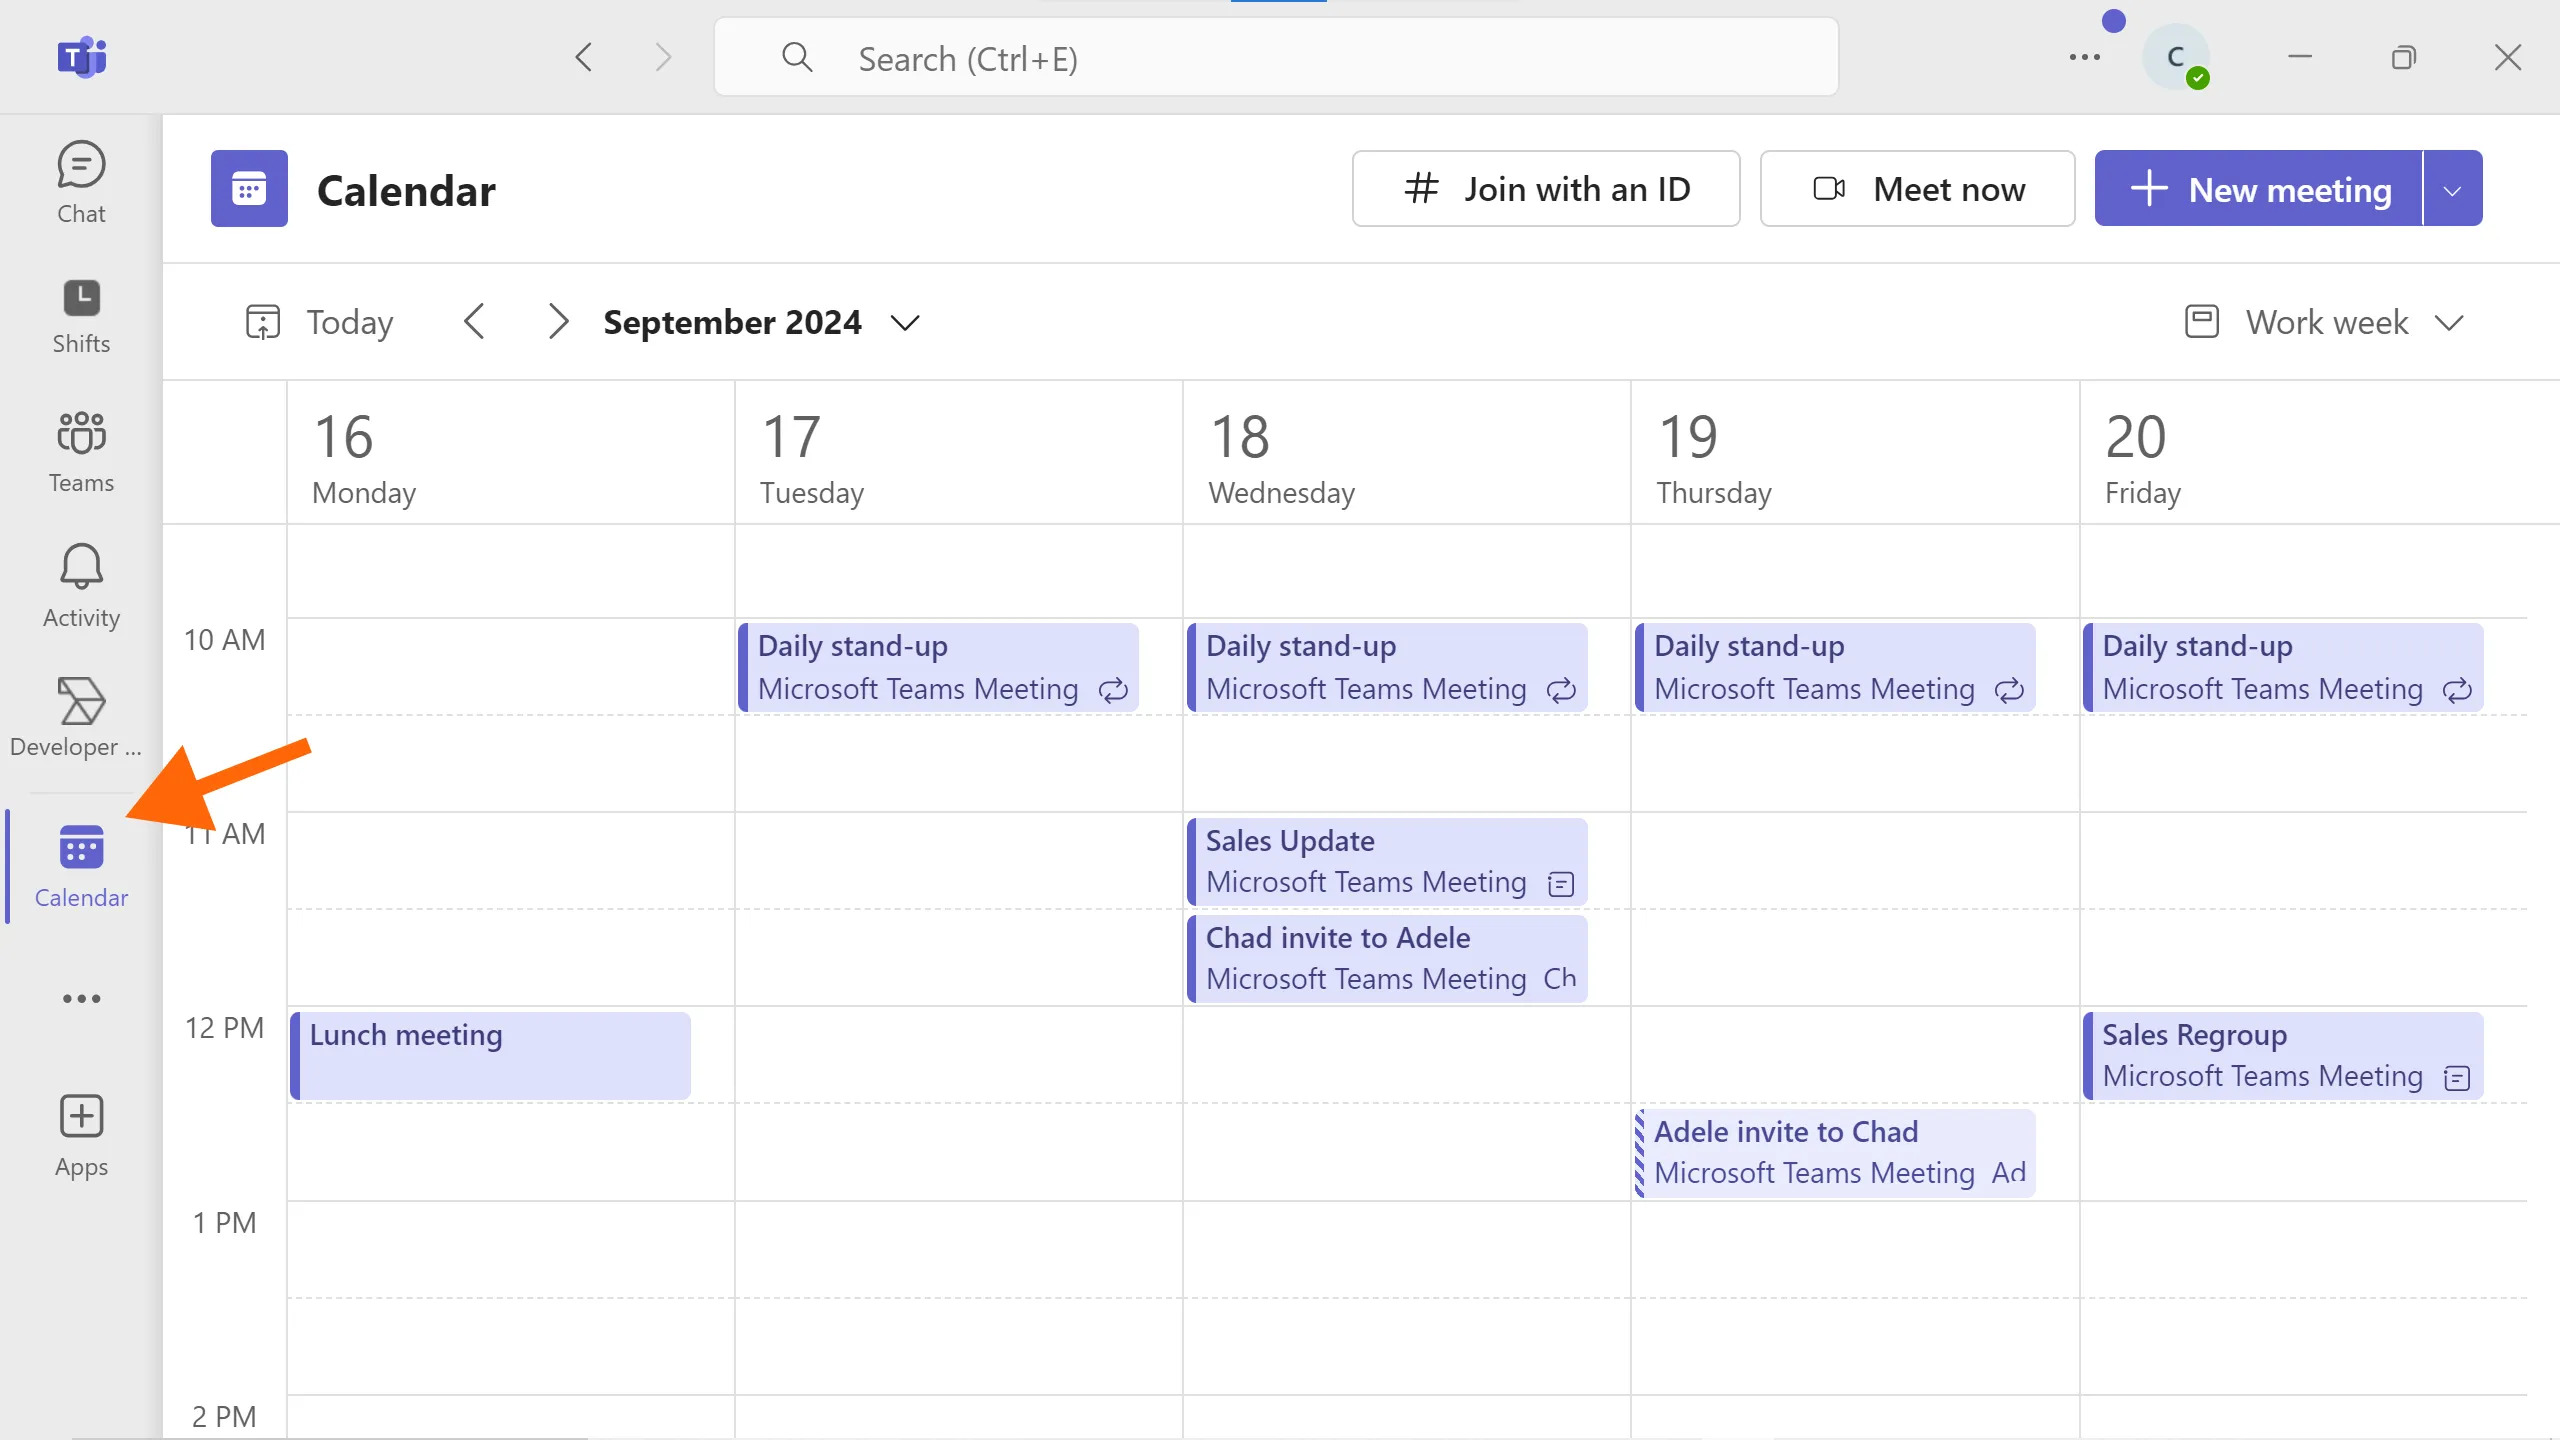
\includegraphics[width=0.6\textwidth]{Teams-calendar.jpg}
  \caption{Exemple illustratif du calendrier Microsoft Teams (source : image libre sur Internet)}
  \label{fig:teamscalendar}
\end{figure}
\subsubsection{Inconvénients de la situation actuelle}
\vspace{0,3cm}
\hspace*{2em}Le dispositif actuel est fonctionnel, mais il peut être nettement amélioré afin de permettre une économie de temps et d’effort, tout en offrant une meilleure expérience utilisateur et d’apprentissage.
Les inconvénients de cette approche sont listés comme suit :
\begin{itemize}
    \item Utilisation de plusieurs plateformes pour la planification : les demandes sont envoyées via Gmail, tandis que les formations sont organisées via Microsoft Teams. Cette séparation demande un effort supplémentaire en termes de coordination et de temps.
    \item Manque de centralisation et d’accessibilité des contenus : les supports de formation sont souvent dispersés entre des e-mails, fichiers PDF et documents partagés, ce qui rend leur recherche difficile, notamment pour les formations anciennes. De plus, les parcours ne sont ni centralisés ni structurés.
    \item Difficulté d’accès pour les nouveaux employés : il n’est pas facile pour un nouveau employés  de retrouver les supports des formations passées ou d’y accéder rapidement.
    \item Absence de suivi individualisé : Il est difficile d’assurer un suivi personnalisé.
\end{itemize}


\subsection{Étude de solutions existantes}
\hspace*{2em}Ces dernières années, plusieurs solutions ont été développées pour gérer la formation au sein des entreprises. Nous avons analysé certaines d’entre elles afin d’identifier leurs avantages et inconvénients, dans le but de nous en inspirer pour construire une solution plus adaptée à nos besoins.

\hspace{1cm}

\noindent \textbf{LinkedIn Learning \cite{Linkedin-Learning}:}

\vspace{0.3cm}

Il s’agit d’une fonctionnalité intégrée à LinkedIn, conçue spécifiquement pour les entreprises. Celles-ci paient des frais d’abonnement pour permettre à leurs employés d'accéder à un large catalogue de cours dispensés par des experts certifiés et des formateurs professionnels.

\vspace{0.3cm}

\begin{figure}[h!]
  \centering
  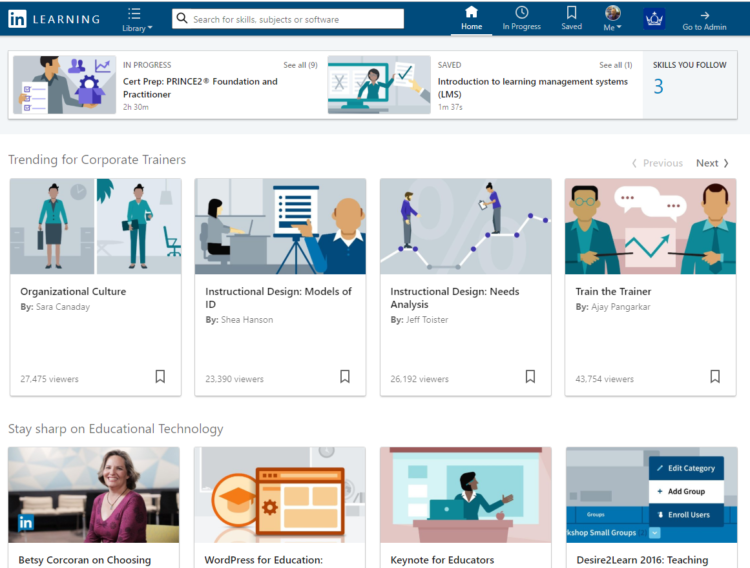
\includegraphics[width=0.6\textwidth]{linkedin-learning.png}
  \caption{ Accueil de la plateforme LinkedIn Learning}
  \label{fig:linkedin-learning}
\end{figure}

\vspace{0.3cm}

\noindent Inconvénients :

\vspace{0.3cm}

Malgré la richesse des contenus, LinkedIn Learning ne permet pas aux entreprises de créer leurs propres cours privés ou formations spécifiques pour leurs équipes. Il n’existe pas d’espace personnalisé pour chaque entreprise : le contenu est global et partagé selon le principe du "tout le monde peut voir tout". Ce manque de personnalisation et de confidentialité peut être un frein pour certaines organisations.

\vspace{1cm}

\noindent \textbf{Udemy Business \cite{Udemy}:}

\vspace{0.3cm}

Il s'agit de la version professionnelle de la plateforme Udemy, destinée aux entreprises souhaitant former leurs employés. Elle donne accès à un catalogue varié de cours (technologie, management, soft skills, etc.).

\noindent Les entreprises peuvent importer leurs propres contenus (vidéos, documents, etc.).De plus, l’accès est limité aux utilisateurs ayant un compte d’entreprise, ce qui garantit une certaine confidentialité, 
Cette flexibilité et cette confidentialité sont des avantages importants dont LinkedIn Learning ne dispose pas.

\vspace{0.3cm}

\begin{figure}[H]
  \centering
  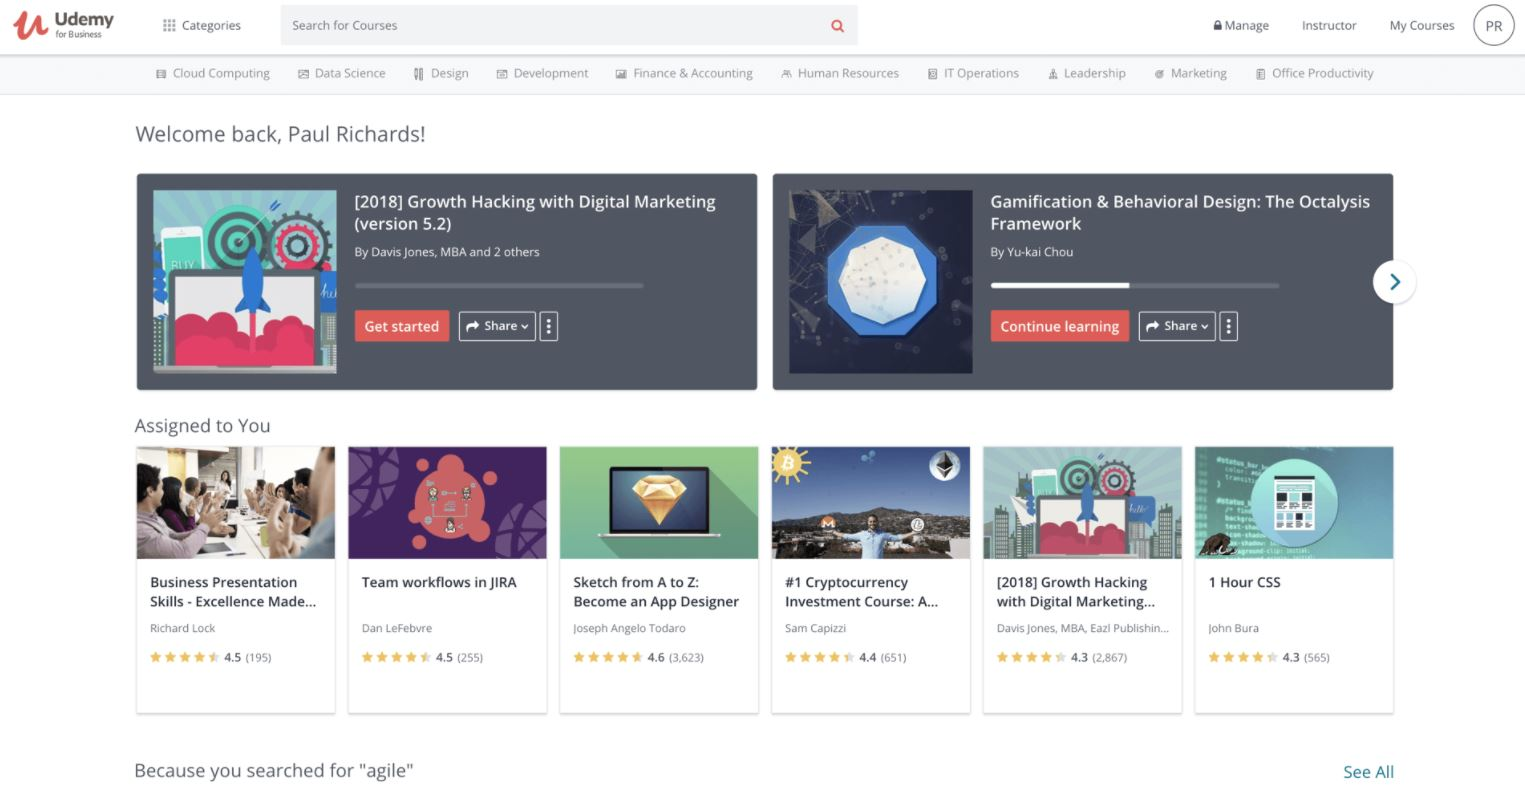
\includegraphics[width=0.6\textwidth]{udemy-business.jpg}
  \caption{Udemy Business}
  \label{fig:Udemy-Business}
\end{figure}

\vspace{0.3cm}

\noindent Inconvénients :

\vspace{0.3cm}

Udemy propose un abonnement qui donne accès à l'ensemble de ses fonctionnalités. Il existe de nombreuses plateformes ayant un modèle similaire à celui d'Udemy Business, comme TalentLMS et Coursera for Business. Cependant, pour une entreprise cherchant à sélectionner les meilleures solutions tout en minimisant les coûts et le temps, et visant à être indépendante d'autres plateformes (afin d'éviter que d'éventuelles pannes de ces plateformes n'impactent le processus d'apprentissage au sein de l'organisation ), ces dernières ne répondent pas entièrement à leurs attentes.


\subsection{Résumé de la solution envisagée}

\vspace{0.5cm}

\hspace*{2em}Après avoir analysé la situation actuelle de la gestion des formations au sein de l’entreprise, et étudié plusieurs plateformes e-learning disponibles sur le marché pouvant constituer des solutions, nous avons identifié certaines limitations dans ces plateformes
\begin{itemize}
    \item l’incapacité à créer du contenu personnalisé
    \item le manque d’indépendance pour l’entreprise
    \item les frais d’abonnement parfois élevés, etc.
\end{itemize}

 \noindent Ces remarques nous conduisent à recommander une approche plus personnalisée et appropriée.
Une plateforme de e-learning privée pour la gestion des formations, qui va permettre de : 
\begin{itemize}
    \item Minimiser les coûts à long terme.
    \item Contrôler et personnaliser totalement les contenus.
    \item Simplifier l'accès aux ressources de formation.
    \item Être indépendante technologiquement.
    \item Gérer la planification des formations et faciliter le processus pour l’équipe de ressources humaines et pour les formateurs (professeurs). 
\end{itemize}
\newpage
\section{La Conception}
\vspace{1cm}

\hspace*{2em}Après avoir effectué nos études et recherches, nous avons conçu une plateforme d’e-learning privée appelée "\textbf{TAKWINI}" destinée à faciliter l’apprentissage au sein de GIG Algeria.

\vspace{0,3cm}

\noindent Ce chapitre va présenter les caractéristiques qui ont permis d'atteindre les objectifs fixés dans le chapitre précédent, ainsi que d'autres fonctionnalités développées pour répondre aux problèmes relevés antérieurement. Nous discuterons également de la conception technique et fonctionnelle de cette plateforme.

\vspace{0,2cm}
\subsection{Fonctionnalités principales}


\vspace{0,2cm}
L'ensemble des utilisateurs se compose d'employés, de professeurs et d'administrateurs.
\begin{itemize}
    \item La plateforme est privée : toute personne non autorisée ne peut pas y accéder. Elle est donc sécurisée et personnalisée, exclusivement destinée au personnel de GIG Algeria.


    \item Elle offre une gestion complète des comptes afin d’atteindre le niveau de personnalisation souhaité. De plus, la gestion des conférences est assurée par les administrateurs de la plateforme pour une planification structurée.
    

 \item La plateforme repose sur une gestion des rôles combinant le département et la fonction de l’utilisateur, ce qui permet d’attribuer à chacun un espace personnalisé.
\item Elle propose un apprentissage facilité grâce à la disponibilité de toutes les ressources pédagogiques, ainsi qu’un accès simplifié à celles-ci. 
\item L’utilisateur peut être informé de la programmation de l’ensemble des conférences, qu’elles soient en ligne ou en présentiel. Il peut également assister aux conférences en ligne.





    
    \item Il est possible de suivre sa progression personnelle.
   
\end{itemize}

\noindent L’ensemble de ces fonctionnalités a été pensé pour rendre l’expérience d’apprentissage fluide, accessible et adaptée aux besoins internes de l’entreprise.
\subsection{Définition UML} 
\hspace*{2em}Le langage UML (Unified Modeling Language, ou langage de modélisation unifié) a été pensé pour être un langage de modélisation visuelle commun, et riche sémantiquement et syntaxiquement. Il est destiné à l'architecture, la conception et la mise en œuvre de systèmes logiciels complexes par leur structure aussi bien que leur comportement. L'UML a des applications qui vont au-delà du développement logiciel, notamment pour les flux de processus dans l'industrie.\cite{UML}
\subsubsection{Définition d'un acteur}
\hspace*{2em}Chaque acteur joue dans le système un rôle spécifique, que l'on appelle un cas d'utilisation. Plusieurs acteurs peuvent réaliser un même cas d'utilisation. Par acteur, l'on entend aussi bien une personne, un client par exemple, qu'un ordinateur, un système de bases de données par exemple, ou encore un serveur.\cite{Acteur}

\begin{itemize}


\item Employé : un utilisateur de la plateforme ayant pour rôle principal de suivre des formations.

\item Professeur : formateur interne chargé d’animer des formations.

\item Administrateur : responsable de la gestion de la plateforme.
\end{itemize}
\subsubsection{Définition du diagramme de cas d’utilisation}


\hspace*{2em}Un use case, ou cas d'utilisation, est une description claire et précise des interactions entre un utilisateur (ou un autre acteurs systeme) et un système informatique pour atteindre un objectif spécifique. Introduit par Ivar Jacobson dans les années 80, il est couramment utilisé dans la methode analyse conception en Unified Modeling Language (UML)..\cite{Usecase}

\subsubsection{Les diagrammes de cas d'utilisation}

\vspace{0,5cm}
 \hspace*{2em} Dans notre conception, nous avons réalisé quatre diagrammes de cas d’utilisation : un diagramme global qui présente les principales fonctionnalités de chaque rôle, et trois diagrammes détaillés permettant d’expliquer plus précisément le fonctionnement du système.
\begin{center}
     \textbf{\textit{Global}}
\end{center}
\begin{figure}[H]
  \centering
  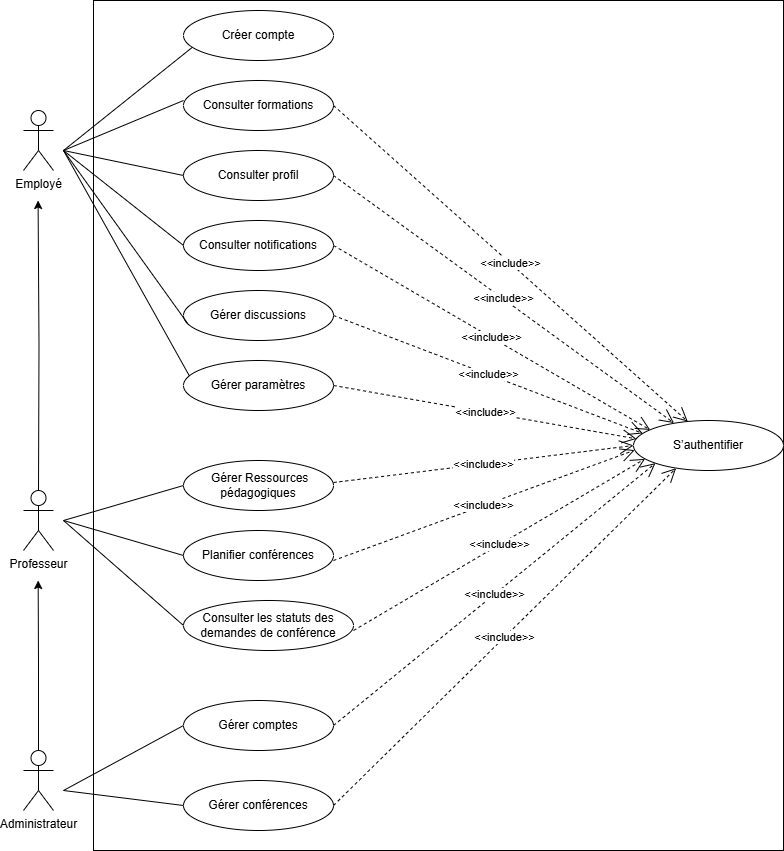
\includegraphics[width=0.6\textwidth]{global(1.2).drawio.png}
  \caption{Diagramme de cas d’utilisation global}
  \label{fig:globalusecase}
\end{figure}
Ce diagramme de cas d’utilisation global présente les principales interactions entre les utilisateurs de la plateforme et le système. Trois rôles principaux sont identifiés : Employé, Professeur, et Administrateur.
\begin{itemize}

\item Employé : peut s’inscrire, consulter les formations, son profil, les notifications ainsi que Gérer ses messages et paramètres.
\item Professeur : possède les mêmes droits qu’un employé, et peut en plus gérer ses ressources pédagogique, planifier des conférences et consulter leur état d’acceptation.
\item Administrateur : dispose de l’ensemble des droits, incluant la gestion des comptes utilisateurs et des conférences.

\end{itemize}

\noindent La création du tout premier compte (celui du directeur des ressources humaines) est effectuée manuellement par nos soins. Ensuite, les utilisateurs s’inscrivent via un formulaire, soumis à validation par l’administration.
\newpage
\begin{center}
     \textbf{\textit{Employé}}
\end{center}
\begin{figure}[H]
  \centering
  \includegraphics[width=0.6\textwidth]{employé(1.4).drawio.png}
  \caption{Diagramme de cas d'utilisation pour un employé}
  \label{fig:employéusecase}
\end{figure}









Ce cas d’utilisation détaille le fonctionnement du rôle Employé :
\begin{itemize}
    \item Créer un compte.
    \item Consulter les formations :  L’employé peut consulter uniquement les formations de son propre département.

Exemple : si l’employé travaille dans le département IT, il ne verra que les formations liées à ce département.
Les formations sont composées de deux parties :
\begin{itemize}
    \item Les conférences : elles peuvent être en ligne ou en présentiel, organisées par un professeur.
    
Si la conférence est en ligne, l’employé peut y accéder depuis la plateforme via un lien (Lien Teams partagé par le professeur).

    \item Les ressources pédagogiques: ce sont des supports pédagogiques (vidéos, PDF, liens additionnels, etc.). Ces cours peuvent être :
    \begin{itemize}
        \item des supports liés à une conférence,
        \item ou des ressources que le professeur juge utiles à partager.
    \end{itemize}
\end{itemize}
    


\item Consulter son profil :
L’employé peut visualiser ses informations personnelles (nom, e-mail, etc.).

Il peut également consulter sa progression sur la plateforme .












\item Gérer les discussions :
L’employé peut envoyer et recevoir des messages avec tout les utilisateurs.





\item Gérer ses paramètres : Modifier ses informations personnelles (ex : numéro de téléphone, mot de passe).


\end{itemize}
\newpage
\begin{center}
     \textbf{\textit{Professeur (Formateur)}}
\end{center}
\begin{figure}[H]
  \centering
  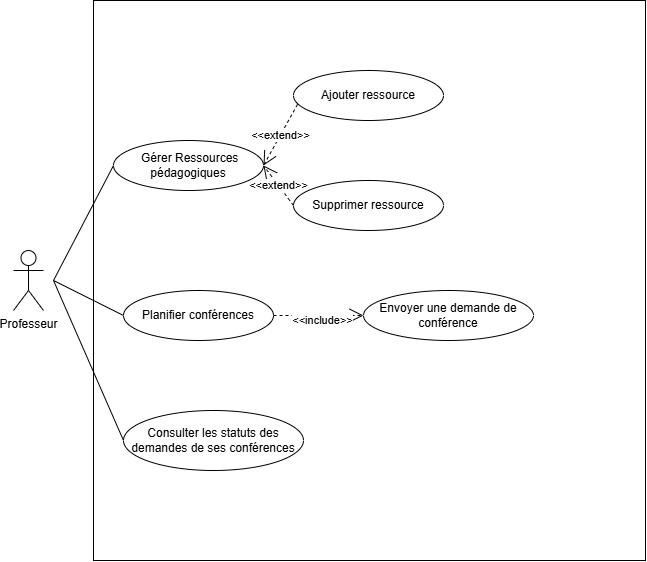
\includegraphics[width=0.6\textwidth]{prof(1.1).drawio.png}
  \caption{Diagramme de cas d'utilisation pour un professeur}
  \label{fig:profusecase}
\end{figure}
Dans ce diagramme, on représente les fonctionnalités du professeur.

\vspace{0,3cm}

\hspace*{2em} Le professeur dispose de toutes les fonctionnalités d’un employé, mais il possède également des droits supplémentaires.
\begin{itemize}
    \item Consultation des formations : 
Le professeur peut consulter les formations de tous les départements (Marketing, IT, Comptabilité, etc.), contrairement à l’employé qui ne voit que celles de son propre département.


\item Gérer ressources pédagogiques : 
Le professeur peut ajouter des ressources pédagogiques, telles que : des vidéos, des fichiers PDF, des liens supplémentaires.
\item Planification de conférences : 
Le professeur peut planifier une conférence, mais cela nécessite d'abord l'envoi d'une demande à l'administration.

La demande doit inclure : la date et l’heure souhaitée, le département concerné, etc.
\item Consulter les statuts des demandes de ses conférences : il peut voir la liste de ses demandes et suivre l’état de chacune.




\end{itemize}

\begin{center}
     \textbf{\textit{Administrateur}}
\end{center}

\begin{figure}[H]
  \centering
  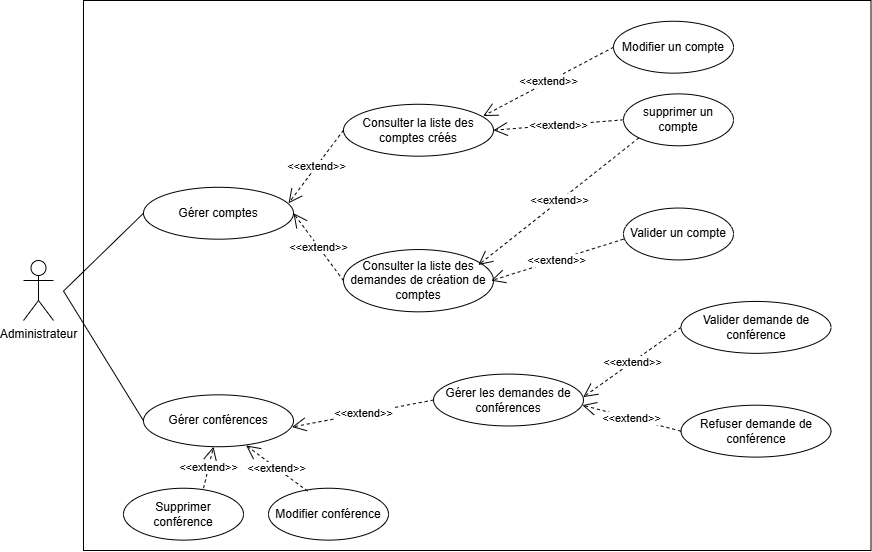
\includegraphics[width=0.6\textwidth]{admin(1.1).drawio.png}
  \caption{Diagramme de cas d'utilisation pour un Administrateur}
  \label{fig:adminusecase}
\end{figure}
\noindent Ce diagramme présente les fonctionnalités supplémentaires de l'administrateur.

\noindent L’administrateur possède toutes les fonctionnalités du professeur, et donc également celles de l’employé. En plus de cela, il dispose de droits d’administration étendus.
\begin{itemize}
    \item Gérer les comptes utilisateurs : il peut consulter la liste des demandes de création de compte utilisateur et les traiter. 

    

L’administrateur peut également consulter la liste des comptes créés, modifier les informations d’un utilisateur (nom, prénom, département, fonction), ou supprimer un compte, par exemple dans le cas d’un employé ayant démissionné.

\item Planification et gestion des conférences : il traite les demandes de conférences envoyées par les professeurs. L’administrateur peut également planifier une conférence , contrairement au professeur, sa demande est automatiquement validée, sans passer par un processus d’approbation. Il peut aussi modifier ou supprimer une conférence déjà programmée, par exemple si un professeur l’annule.




 


    
\end{itemize}

\subsubsection{Définition du diagramme de séquence}






\subsubsection{Les diagrammes de séquence}

\begin{figure}[H]
  \centering
  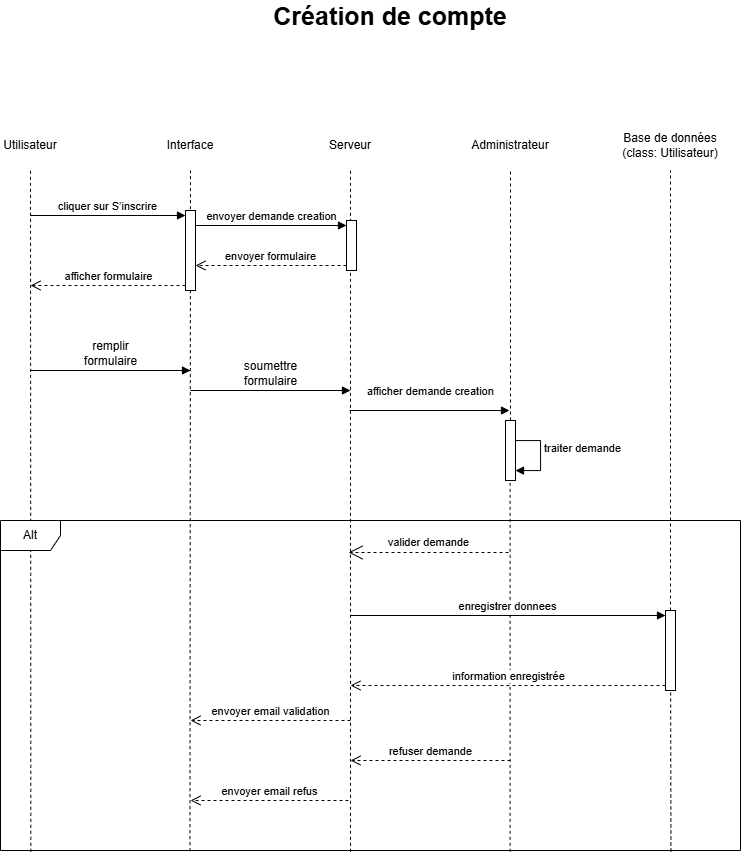
\includegraphics[width=0.6\textwidth]{creationcompte(1.1).drawio.png}
  \caption{Diagramme de Séquence pour la création des comptes}
  \end{figure}
\hspace*{2em} Tous les utilisateurs sont priés de créer un compte sur la plateforme. L’utilisateur clique sur "S’inscrire" et remplit un formulaire dans lequel il précise : son identité, son département, et son rôle (Employé, Professeur ou Administrateur).

\vspace{0,3cm}

\noindent Ce formulaire est ensuite envoyé à l’administration, qui est chargée de le valider. Elle vérifie que l’employé fait bien partie de l’organisation et qu’il appartient au département spécifié.

\vspace{0,3cm}

\noindent Si la vérification est concluante, la demande est validée, le compte est créé et le rôle (département + fonction) est attribué. Sinon, la demande est supprimée.



\begin{figure}[H]
  \centering
  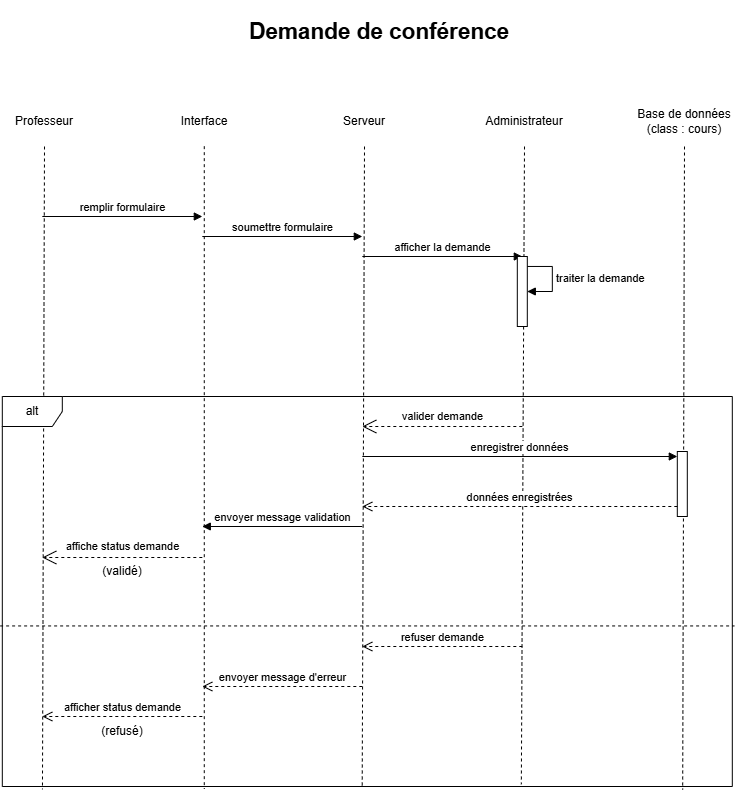
\includegraphics[width=0.6\textwidth]{demandesession(1.1).drawio.png}
  \caption{Diagramme de Séquence pour la demande de conférence}
  \end{figure}

\noindent Lorsque le professeur souhaite planifier une conférence, il remplit un formulaire de demande.

\vspace{0,3cm}

\noindent Une fois la demande envoyée, celle-ci est reçue par l’administrateur, qui consulte le calendrier de la plateforme. Si la date et l’heure demandées sont disponibles, il valide la demande et la conférence est programmée. En cas de conflit avec une conférence déjà prévue à ce moment-là, il refuse la demande. L’état de la demande est ensuite affiché au professeur.

\noindent L’administrateur peut également contacter le professeur pour lui proposer une autre date ou heure disponible.

\vspace{0,5cm}

\noindent Pour voir le diagramme d'authentification, voir l’\hyperref[annexe-auth]{annexe correspondante}.
\subsubsection{Définition du diagramme de classe}

\hspace*{2em} En génie logiciel, un diagramme de classe dans le langage de modélisation unifié (UML) est un type de diagramme de structure statique qui décrit la structure d'un système en montrant les classes du système, leurs attributs, leurs opérations (ou méthodes) et les relations entre les objets. \cite{classe}


\begin{figure}[H]
  \centering
  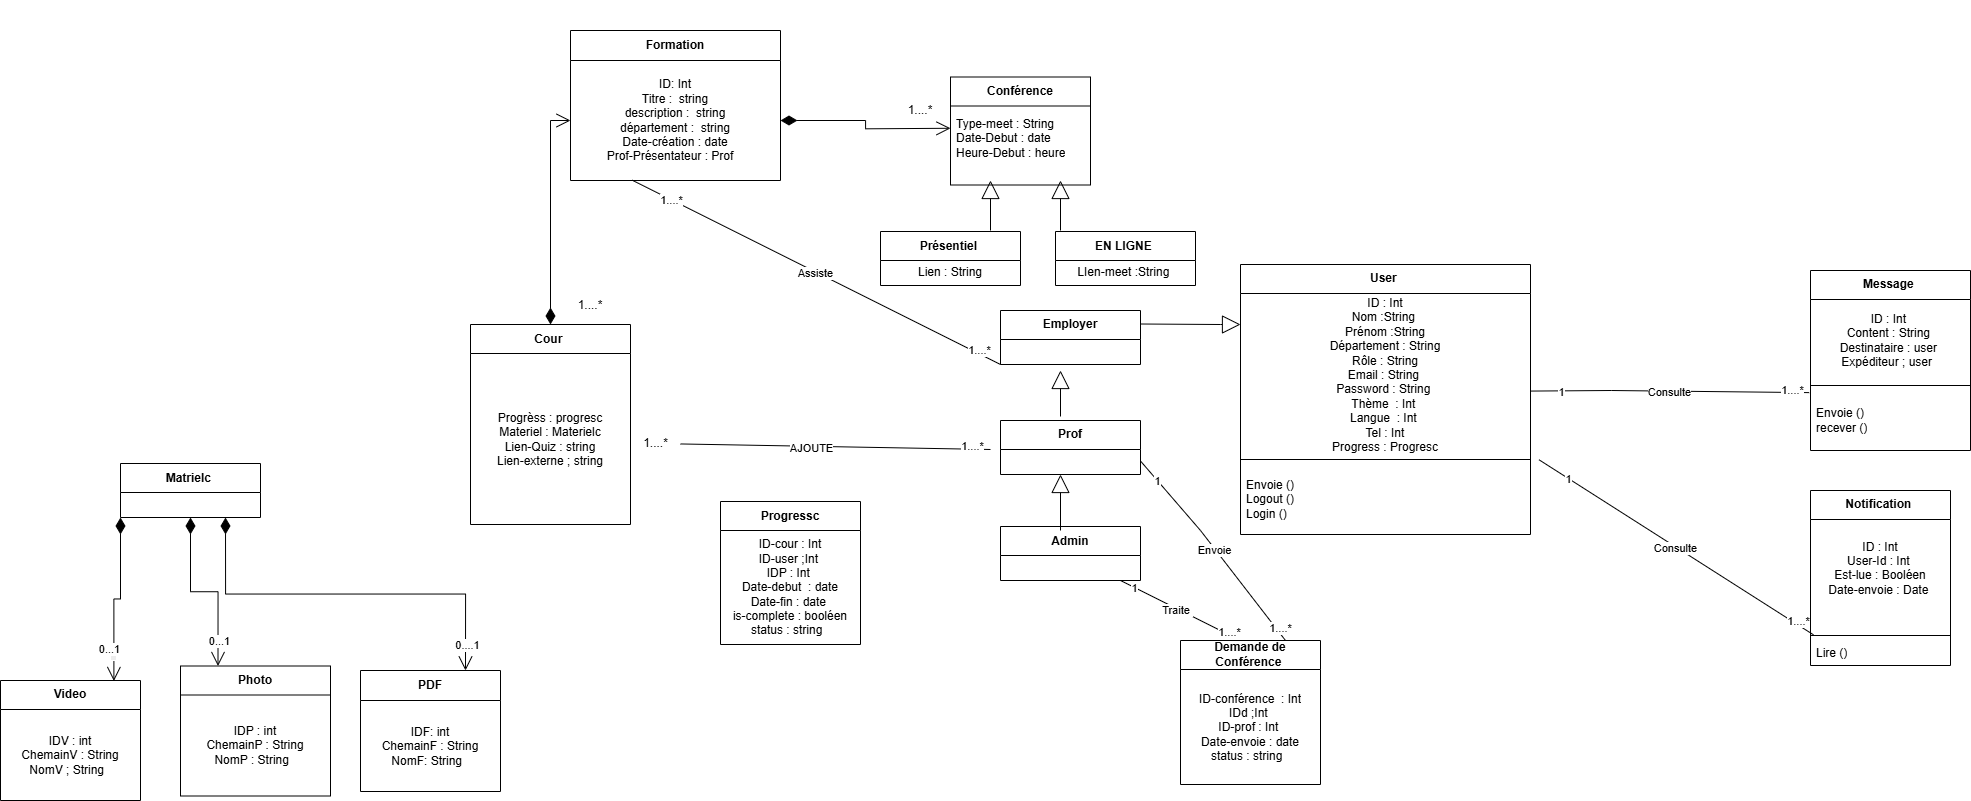
\includegraphics[width=0.9\textwidth]{classe.png}
  \caption{Diagramme de classe}
\end{figure}






\subsection{Définition de design}
\hspace*{2em}Design (ou conception visuelle) désigne le processus de création et d’organisation des éléments graphiques et interactifs d’une application ou d’un site web. Il vise à structurer l’apparence visuelle, l’ergonomie et l’expérience utilisateur (UX), afin de rendre l’interface intuitive, esthétique et fonctionnelle.

\hspace{0,3cm}

\noindent Dans cette phase, nous avons réalisé le design de la plateforme afin de représenter l’apparence visuelle de l’application. Cela nous a permis d’organiser les pages, les boutons, les champs, etc., en tenant compte de l’expérience utilisateur (UX).
\subsubsection{Le design de la plateforme}
\begin{figure}[H]
  \centering
  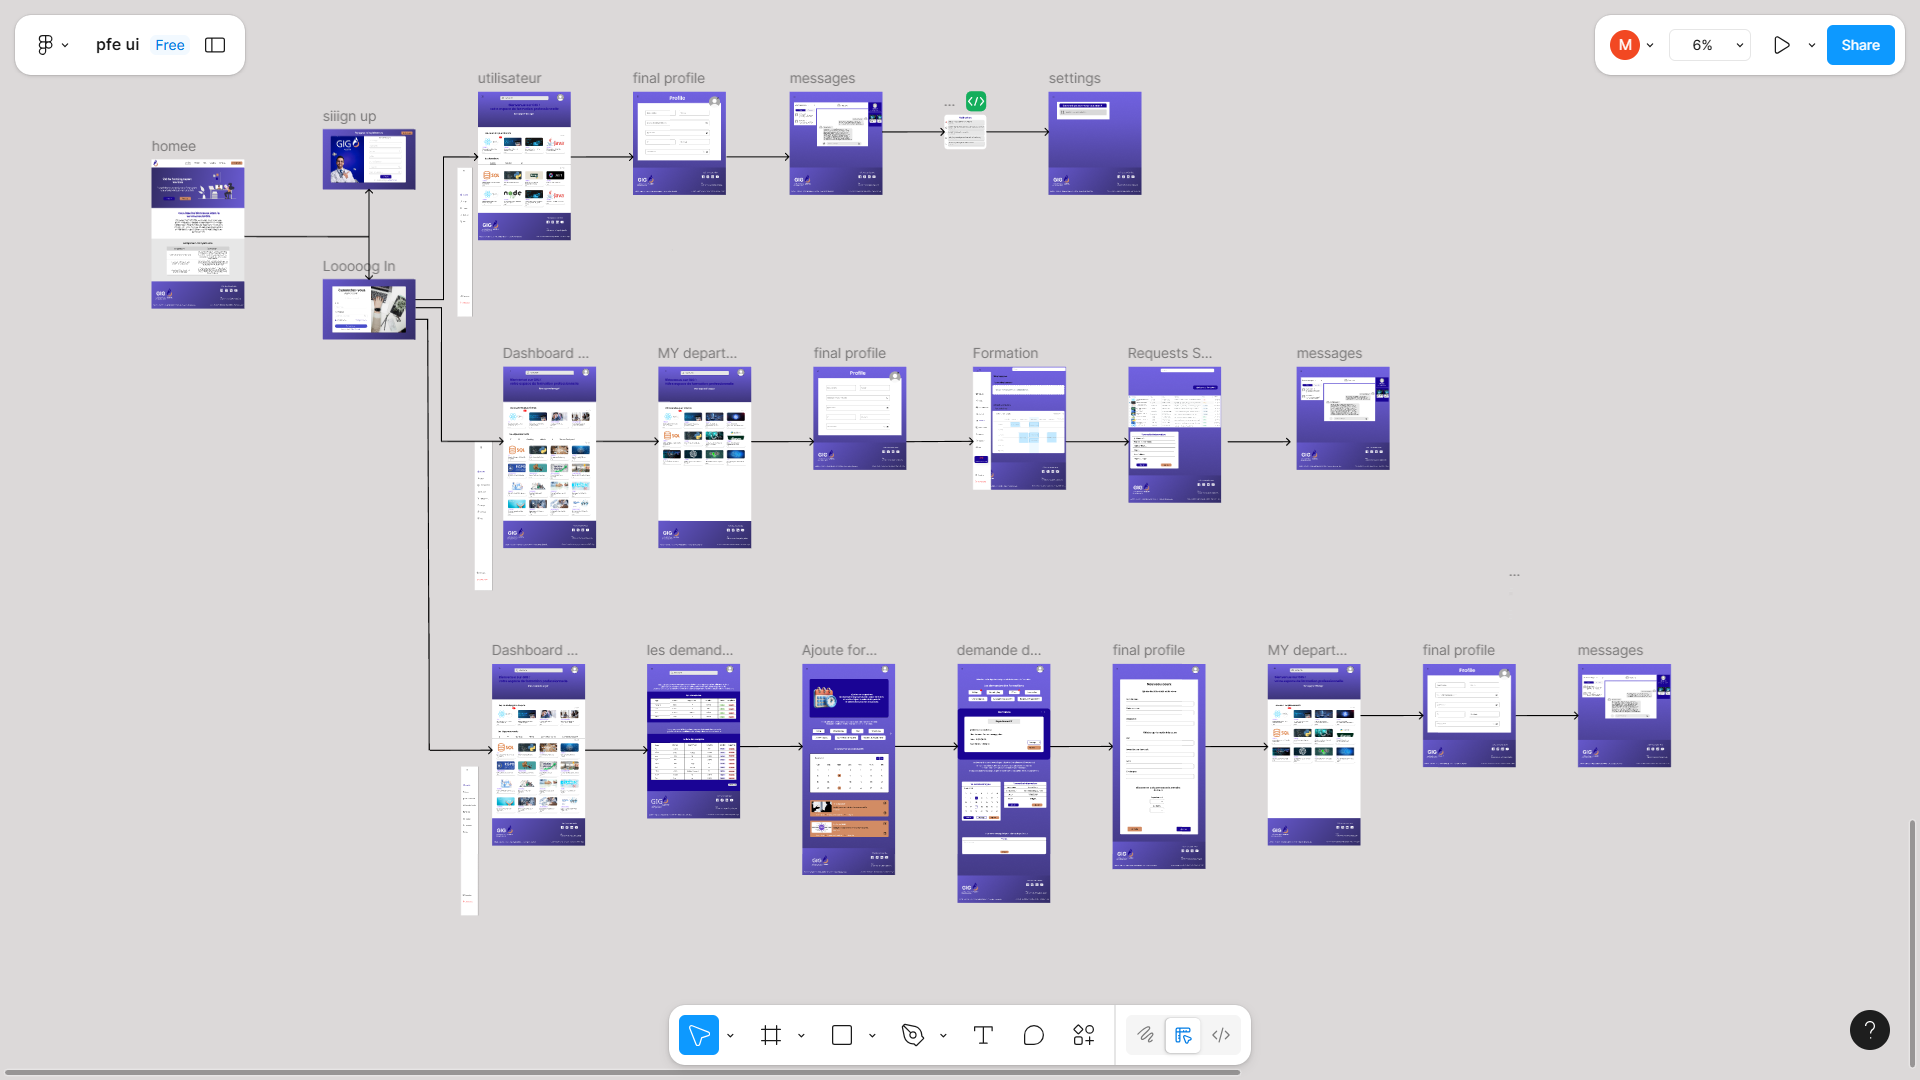
\includegraphics[width=0.6\textwidth]{archifigma.PNG}
  \caption{La hiérarchie de la plateforme}
  \end{figure}

  pour plus de design de plateforme consulter l'\hyperref[annexe-design]{annexe}.


  \newpage
\section{La réalisation pratique}


\hspace*{2em}Dans ce chapitre, nous examinerons les différentes phases de la création de la plateforme « TAKWINI ». Nous identifierons les outils et les langages de programmation employés pour réaliser ce projet, en précisant les raisons qui ont motivé ces choix. Enfin, nous proposerons un aperçu de la plateforme.

\noindent Les phases de réalisation sont : la conception, le développement.
\subsection{Méthodologie adoptée}

\hspace*{2em}Dans le but d'assurer la bonne réalisation de notre plateforme, nous avons décidé d'adopter la méthode du cycle en V. Cette approche nous a permis de structurer clairement les étapes du projet.

\noindent Le cycle en V consiste en une série de phases linéaires qui se succèdent l'une après l'autre jusqu'à ce que le projet soit terminé. La partie gauche du cycle en V énumère les phases de conception et vérification du développement. La partie droite énumère les phases de validation parallèles du développement.

\noindent En suivant la méthodologie du cycle en V, nous avons organisé notre travail en plusieurs étapes distinctes :
\begin{itemize}
    \item L’étude des besoins 
    \item La conception
    \item Le développement
    \item Les tests
\end{itemize}

\subsection{Les outils utilisés dans la conception}
Le logiciel utilisé pour modéliser les différents diagrammes nécessaires à la conception de la plateforme est Draw.io.




\vspace{0,5cm}

\noindent \textbf{Draw.io \cite{drawiointerface}: }

\noindent
\begin{tabular}
{@{}m{0.8\textwidth}@{\hspace{1em}}m{0.2\textwidth}@{}}
Draw.io est une application gratuite en ligne, accessible via son navigateur (protocole https) qui permet de dessiner des diagrammes ou des organigrammes.  
Cet outil propose de concevoir toutes sortes de diagrammes, de dessins vectoriels, de les enregistrer au format XML puis de les exporter.  
Draw.io est un véritable couteau suisse de la frise chronologique, de la carte mentale et des diagrammes de tout genre.\cite{draw-io}
&

\includegraphics[width=\linewidth]{drawio (2).png} % <-- adapte ici le nom réel de ton fichier
\end{tabular}

\noindent La raison de ce choix est que Draw.io est un outil gratuit, directement accessible depuis un navigateur, et ne nécessitant aucun compte pour être utilisé. Il offre toutes les fonctionnalités dont nous avons besoin pour créer des diagrammes clairs et professionnels. De plus, son interface est simple, ce qui le rend facile à comprendre et à utiliser.




\vspace{1cm}

\noindent La conception de l’interface utilisateur (UI) de la plateforme a été réalisée avec Figma.

\vspace{0,5cm}

\noindent \textbf{Figma \cite{figmainterface}: }

\noindent
\begin{tabular}
{@{}m{0.8\textwidth}@{\hspace{1em}}m{0.2\textwidth}@{}}
Figma est un outil de conception d’interface utilisateur (UI), principalement utilisé pour le prototypage et la collaboration. Entièrement basé sur le web, Figma s’exécute directement dans un navigateur, sans nécessiter de téléchargement ni d’installation.
Il s’agit de l’un des outils de conception les plus accessibles et conviviaux du marché, ce qui le rend très populaire auprès des graphistes, marketeurs, concepteurs UI et UX, quel que soit leur niveau d’expérience.\cite{figma}
&

\includegraphics[width=\linewidth]{Figma.png} % <-- adapte ici le nom réel de ton fichier
\end{tabular}

\noindent Nous avons utilisé Figma car il est simple à apprendre et à maîtriser pour la conception UI/UX. Grâce à ses outils intuitifs, il offre un large espace d’inspiration via la Figma Community. De plus, ses fonctionnalités avancées de collaboration nous permettent de travailler efficacement en équipe.



\subsection{Le développement}

\hspace*{2em}L'objectif de cette étape est de transformer les maquettes, diagrammes et spécifications établies lors de la phase de conception en une application opérationnelle. Nous présentons ici l’architecture logicielle adoptée, les langages et technologies utilisés, ainsi que les différentes fonctionnalités implémentées.


\subsubsection{Architecture adoptée}
\hspace*{2em}L’architecture adoptée pour le développement de TAKWINI est une architecture \textbf{client-serveur}, caractérisée par une séparation entre le frontend et le backend.

\vspace{0,3cm}

\noindent \hyperref[annexe-client-ser]{Définition de l’architecture client-serveur}.

\vspace{0,3cm}

\noindent
\begin{tabular}
{@{}m{0.8\textwidth}@{\hspace{1em}}m{0.2\textwidth}@{}}
Dans la phase de développement, nous avons utilisé l’éditeur Visual Studio Code car il offre la possibilité de travailler simultanément sur plusieurs onglets et fenêtres, ce qui améliore considérablement la productivité. De plus, il est léger, rapide et dispose de nombreuses fonctionnalités de personnalisation.
&

\includegraphics[width=\linewidth]{images.png} % <-- adapte ici le nom réel de ton fichier
\end{tabular}


\vspace{0,5cm}

\noindent \normalsize \textbf{Github \cite{github}: }

\vspace{0,1cm}

\noindent
\begin{tabular}
{@{}m{0.8\textwidth}@{\hspace{1em}}m{0.17\textwidth}@{}}
GitHub nous permet de déployer notre code, tout en facilitant la collaboration en équipe. Il offre un environnement de travail partagé où chaque membre peut contribuer, suivre les modifications et gérer les versions du projet.


&

\includegraphics[width=\linewidth]{github.png} % <-- adapte ici le nom réel de ton fichier
\end{tabular}

\vspace{0,8cm}

\noindent \large \textbf{Frontend :}

\vspace{0,8cm}


\noindent \normalsize \textbf{HTML :}

\vspace{0,1cm}

\noindent
\begin{tabular}
{@{}m{0.8\textwidth}@{\hspace{1em}}m{0.25\textwidth}@{}}
Nous avons utilisé HTML (HyperText Markup Language) pour définir la structure de base des pages de notre plateforme. Cela inclut l'organisation des sections, des titres, des paragraphes, des boutons, des formulaires et d'autres éléments nécessaires à l'affichage du contenu.
&

\includegraphics[width=\linewidth]{HTML-5-Badge-Logo.png} % <-- adapte ici le nom réel de ton fichier
\end{tabular}

\vspace{0,3cm}

\noindent \normalsize \textbf{CSS :}

\vspace{0,1cm}

\noindent
\begin{tabular}
{@{}m{0.8\textwidth}@{\hspace{1em}}m{0.2\textwidth}@{}}
Nous avons également utilisé CSS (Cascading Style Sheets) pour reproduire le design préalablement conçu. Il nous permet de contrôler l’apparence des éléments d’une page web, notamment la police, les couleurs, les formats, la mise en page, ainsi que l’organisation visuelle souhaitée.


En utilisant CSS, nous avons pu réaliser une version web responsive de la plateforme adaptée à la fois aux écrans d’ordinateur (desktop) et aux téléphones mobiles.
&

\includegraphics[width=\linewidth]{css.png} % <-- adapte ici le nom réel de ton fichier
\end{tabular}


\vspace{0,3cm}


\noindent \normalsize \textbf{Java script :}

\vspace{0,1cm}


\noindent
\begin{tabular}
{@{}m{0.8\textwidth}@{\hspace{1em}}m{0.15\textwidth}@{}}
Dans notre plateforme TAKWINI, JavaScript est utilisé dans le but  de rendre l’interface plus interactive et dynamique. Il permet de manipuler le contenu des pages en temps réel, de gérer les événements utilisateur (clics, saisies, etc.), d’ajouter des animations comme les barres latérales et d’intégrer des services externes via des API, notamment pour l’affichage d’un calendrier interactif.
&

\includegraphics[width=\linewidth]{js.png} % <-- adapte ici le nom réel de ton fichier
\end{tabular}

\noindent \large \textbf{Déploiement du frontend :}

\vspace{0,3cm}

Pour déployer et tester notre code frontend, nous avons utilisé GitHub Pages. Ce service facilite l'hébergement de sites statiques directement depuis un dépôt GitHub, ce qui nous a permis de rendre l'interface de la plateforme accessible en ligne pour les tests et les démonstrations.

\vspace{0,3cm}

\noindent \large \textbf{Backend :}

\vspace{0,5cm}
\newpage

\noindent \large \textbf{FastApi \cite{FastApi}:}

\vspace{0,3cm}

\noindent
\begin{tabular}
{@{}m{0.8\textwidth}@{\hspace{1em}}m{0.15\textwidth}@{}}
Pour le développement du back-end de notre plateforme TAKWINI, nous avons utilisé FastAPI, un framework moderne et rapide basé sur le langage Python. FastAPI est conçu pour la création d'API web performantes, en tirant parti des annotations de type pour simplifier le développement et améliorer la lisibilité du code. Ce framework offre de nombreuses bibliothèques intégrées qui accélèrent le processus de développement. Par exemple, SQLAlchemy, un ORM (Object-Relational Mapping), permet d’intégrer la base de données et de la manipuler à l’aide d’objets Python, au lieu d’écrire directement des requêtes SQL brutes. De même, Python-jose est utilisé pour la gestion des JWT (JSON Web Tokens), ce qui permet de sécuriser la communication entre le client et le serveur, tout en assurant une meilleure gestion des requêtes HTTP, de la validation des données et de la documentation automatique des API. Grâce à sa simplicité et sa performance, FastAPI s’est révélé être un excellent choix pour construire une architecture backend robuste, évolutive et facilement maintenable.

\vspace{0,2cm}

\hspace{0,2cm}pour faciliter le déploiement du back-end, nous avons utilisé la plateforme Render, qui offre une solution simple et efficace pour héberger des applications web.
&

\includegraphics[width=\linewidth]{fastapi.png} % <-- adapte ici le nom réel de ton fichier
\end{tabular}

\vspace{0,8cm}

\noindent \large \textbf {Postgresql \cite{postgresql}:}

\vspace{0,3cm}

\noindent
\begin{tabular}
{@{}m{0.8\textwidth}@{\hspace{1em}}m{0.15\textwidth}@{}}
Nous avons également utilisé PostgreSQL comme système de gestion de base de données relationnelle. Il nous a permis de stocker et d’organiser les données de manière fiable, tout en garantissant l’intégrité et la cohérence des informations. 

la base de données a été déployée sur Railway, une plateforme cloud qui permet une gestion flexible et rapide des bases de données à distance.
Pour l’administration et la visualisation des données, nous avons utilisé pgAdmin 4, un outil graphique qui facilite la gestion des tables, l’exécution de requêtes SQL, et le suivi global de la base de données.
&

\includegraphics[width=\linewidth]{postgre.png} % <-- adapte ici le nom réel de ton fichier
\end{tabular}

\vspace{0,8cm}

\noindent \large \textbf {Cloudinary \cite{cloudinary}:}

\vspace{0,3cm}
\noindent
\begin{tabular}
{@{}m{0.8\textwidth}@{\hspace{1em}}m{0.15\textwidth}@{}}
 La base de données PostgreSQL a été hébergée sur Railway, une solution cloud à la fois simple et efficace. Pour la gestion des fichiers multimédias (PDF, images, vidéos), nous avons intégré Cloudinary, un service de stockage en ligne permettant d’héberger, d’optimiser et de diffuser les fichiers de manière rapide et fiable.
Ce choix a été motivé par le fait que l’entreprise ne pouvait pas nous fournir un accès à son serveur. L’intégration d’un service cloud tel que Cloudinary nous a donc permis d’assurer le bon fonctionnement du système, tout en facilitant le déploiement ainsi que la gestion des fichiers multimédias
 
&

\includegraphics[width=\linewidth]{cloud.png} % <-- adapte ici le nom réel de ton fichier
\end{tabular}




\subsubsection{Interface utilisateur}



\begin{figure}[H]
  \centering
  
\includegraphics[width=0.6\textwidth]{inter.png}
  \caption{L'interface de TAKWINI}
  \label{fig:home}
\end{figure}



\begin{figure}[H]
  \centering
  \begin{subfigure}[t]{0.4\textwidth}
    \centering
    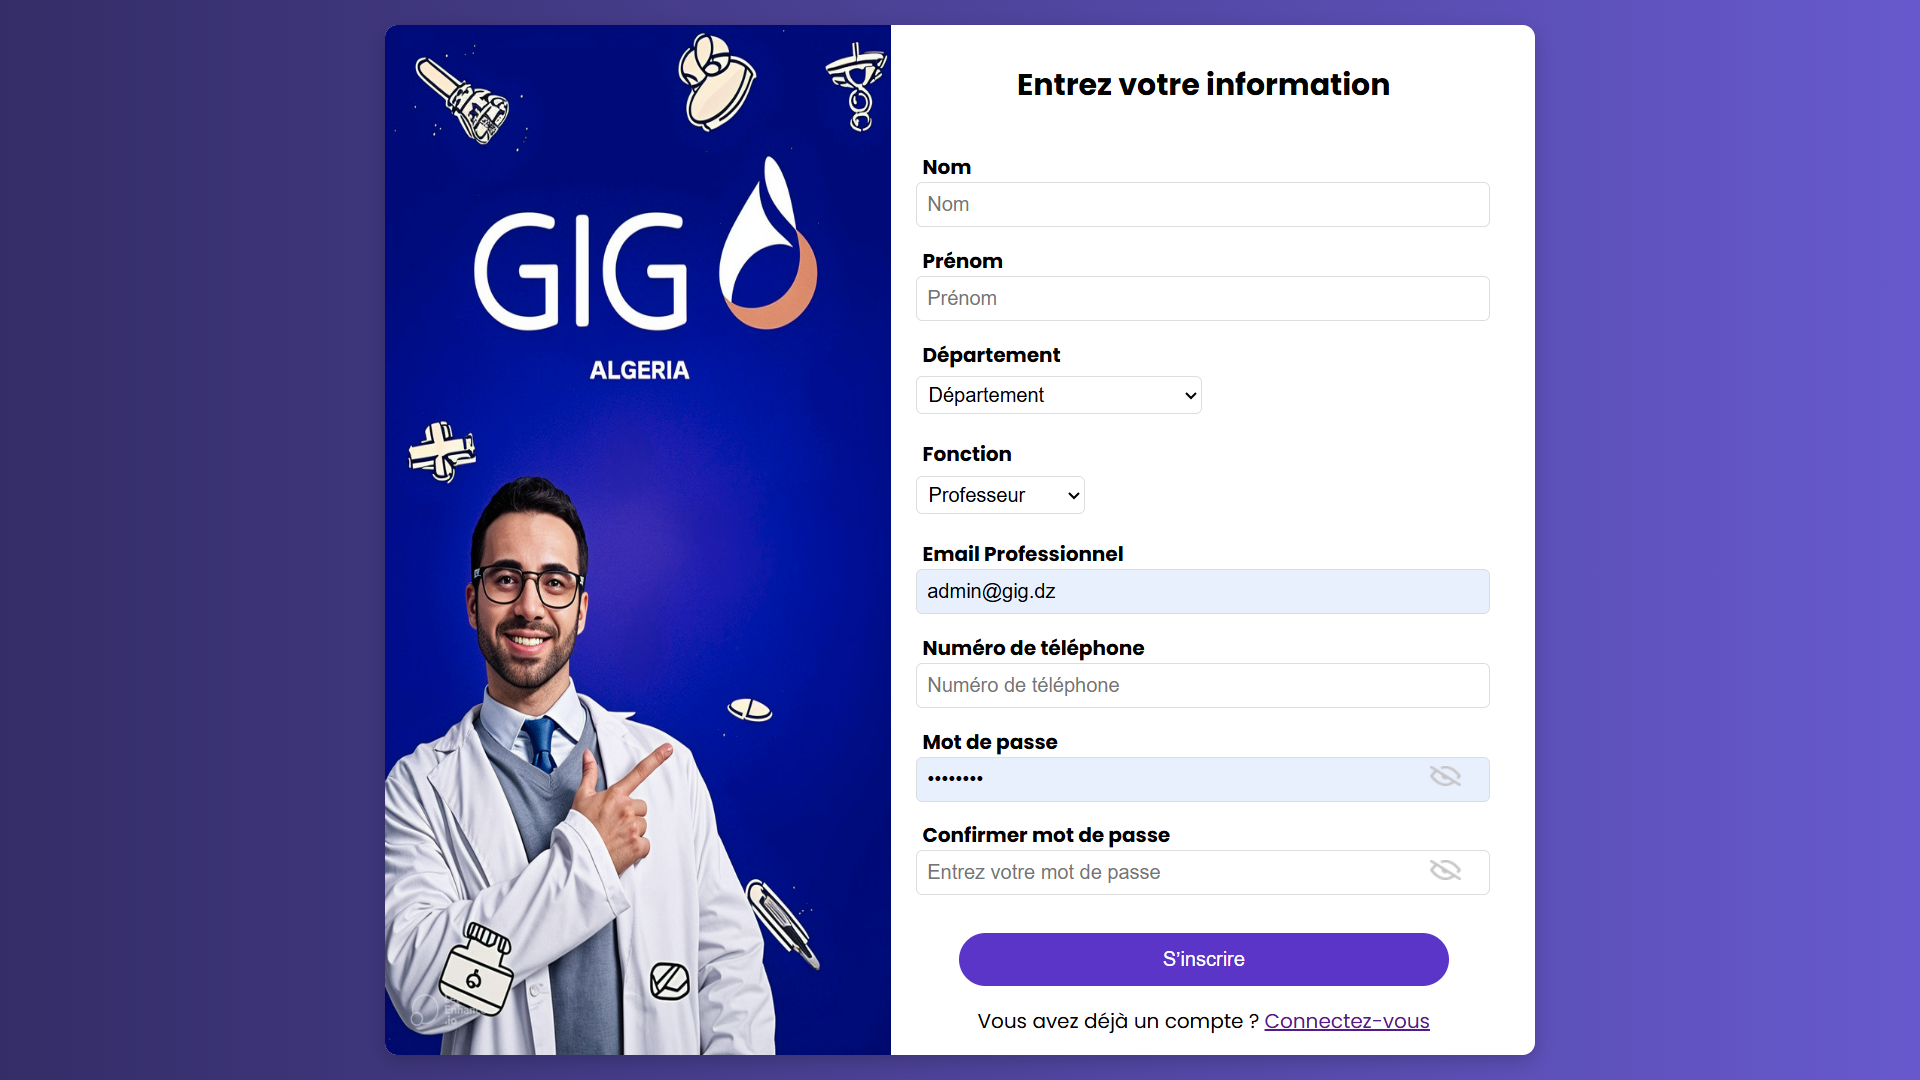
\includegraphics[width=\textwidth]{signup.png}
    \caption{la page d’inscription sur TAKWINI}
    \label{fig:sign-up}
  \end{subfigure}
  \hspace{1cm}
  \begin{subfigure}[t]{0.4\textwidth}
    \centering
    
\includegraphics[width=\textwidth]{login.png}
    \caption{Page de connexion}
    \label{fig:sign-in}
  \end{subfigure}
  \label{fig:login}
\end{figure}

\begin{figure}[H]
  \centering
  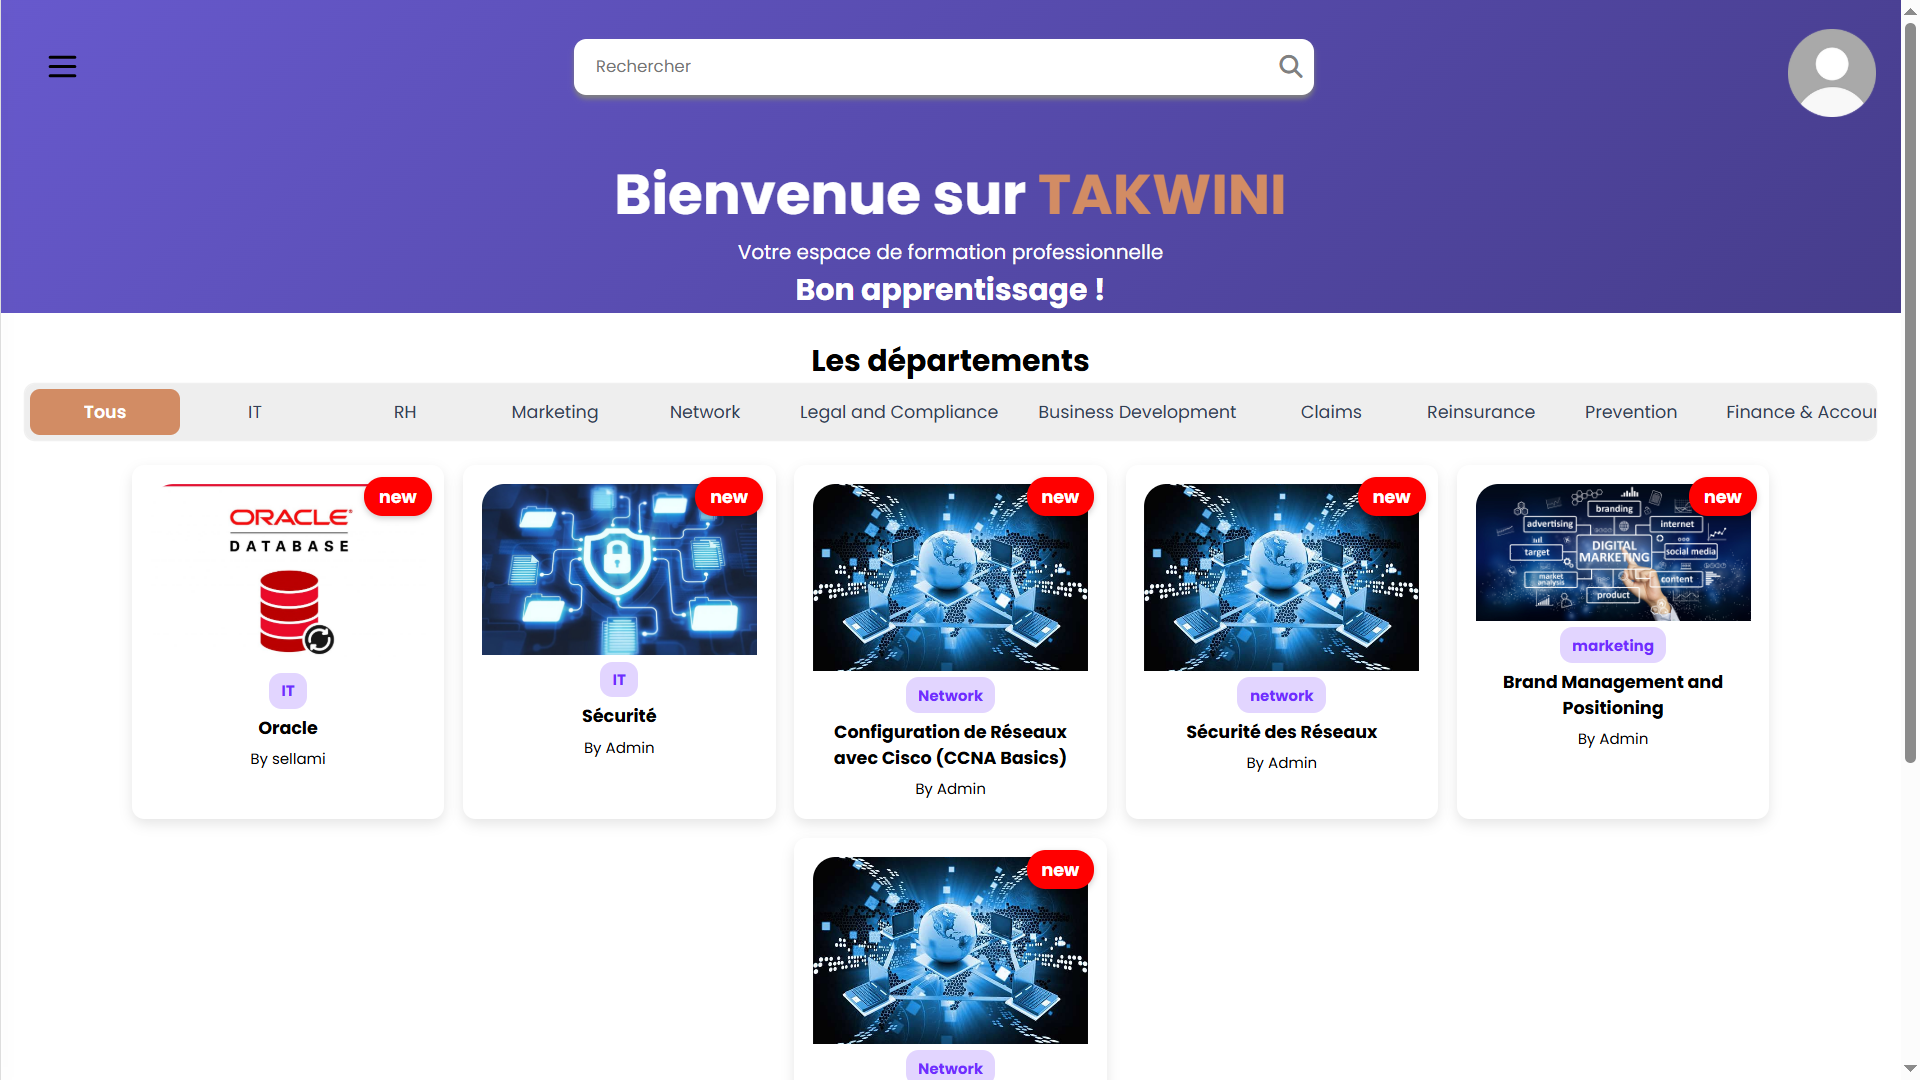
\includegraphics[width=0.6\textwidth]{dashboard.png}
  \caption{Accueil de l'administrateur et professeur}
  \label{fig:dashboard}
\end{figure}



\begin{figure}[H]
  \centering
  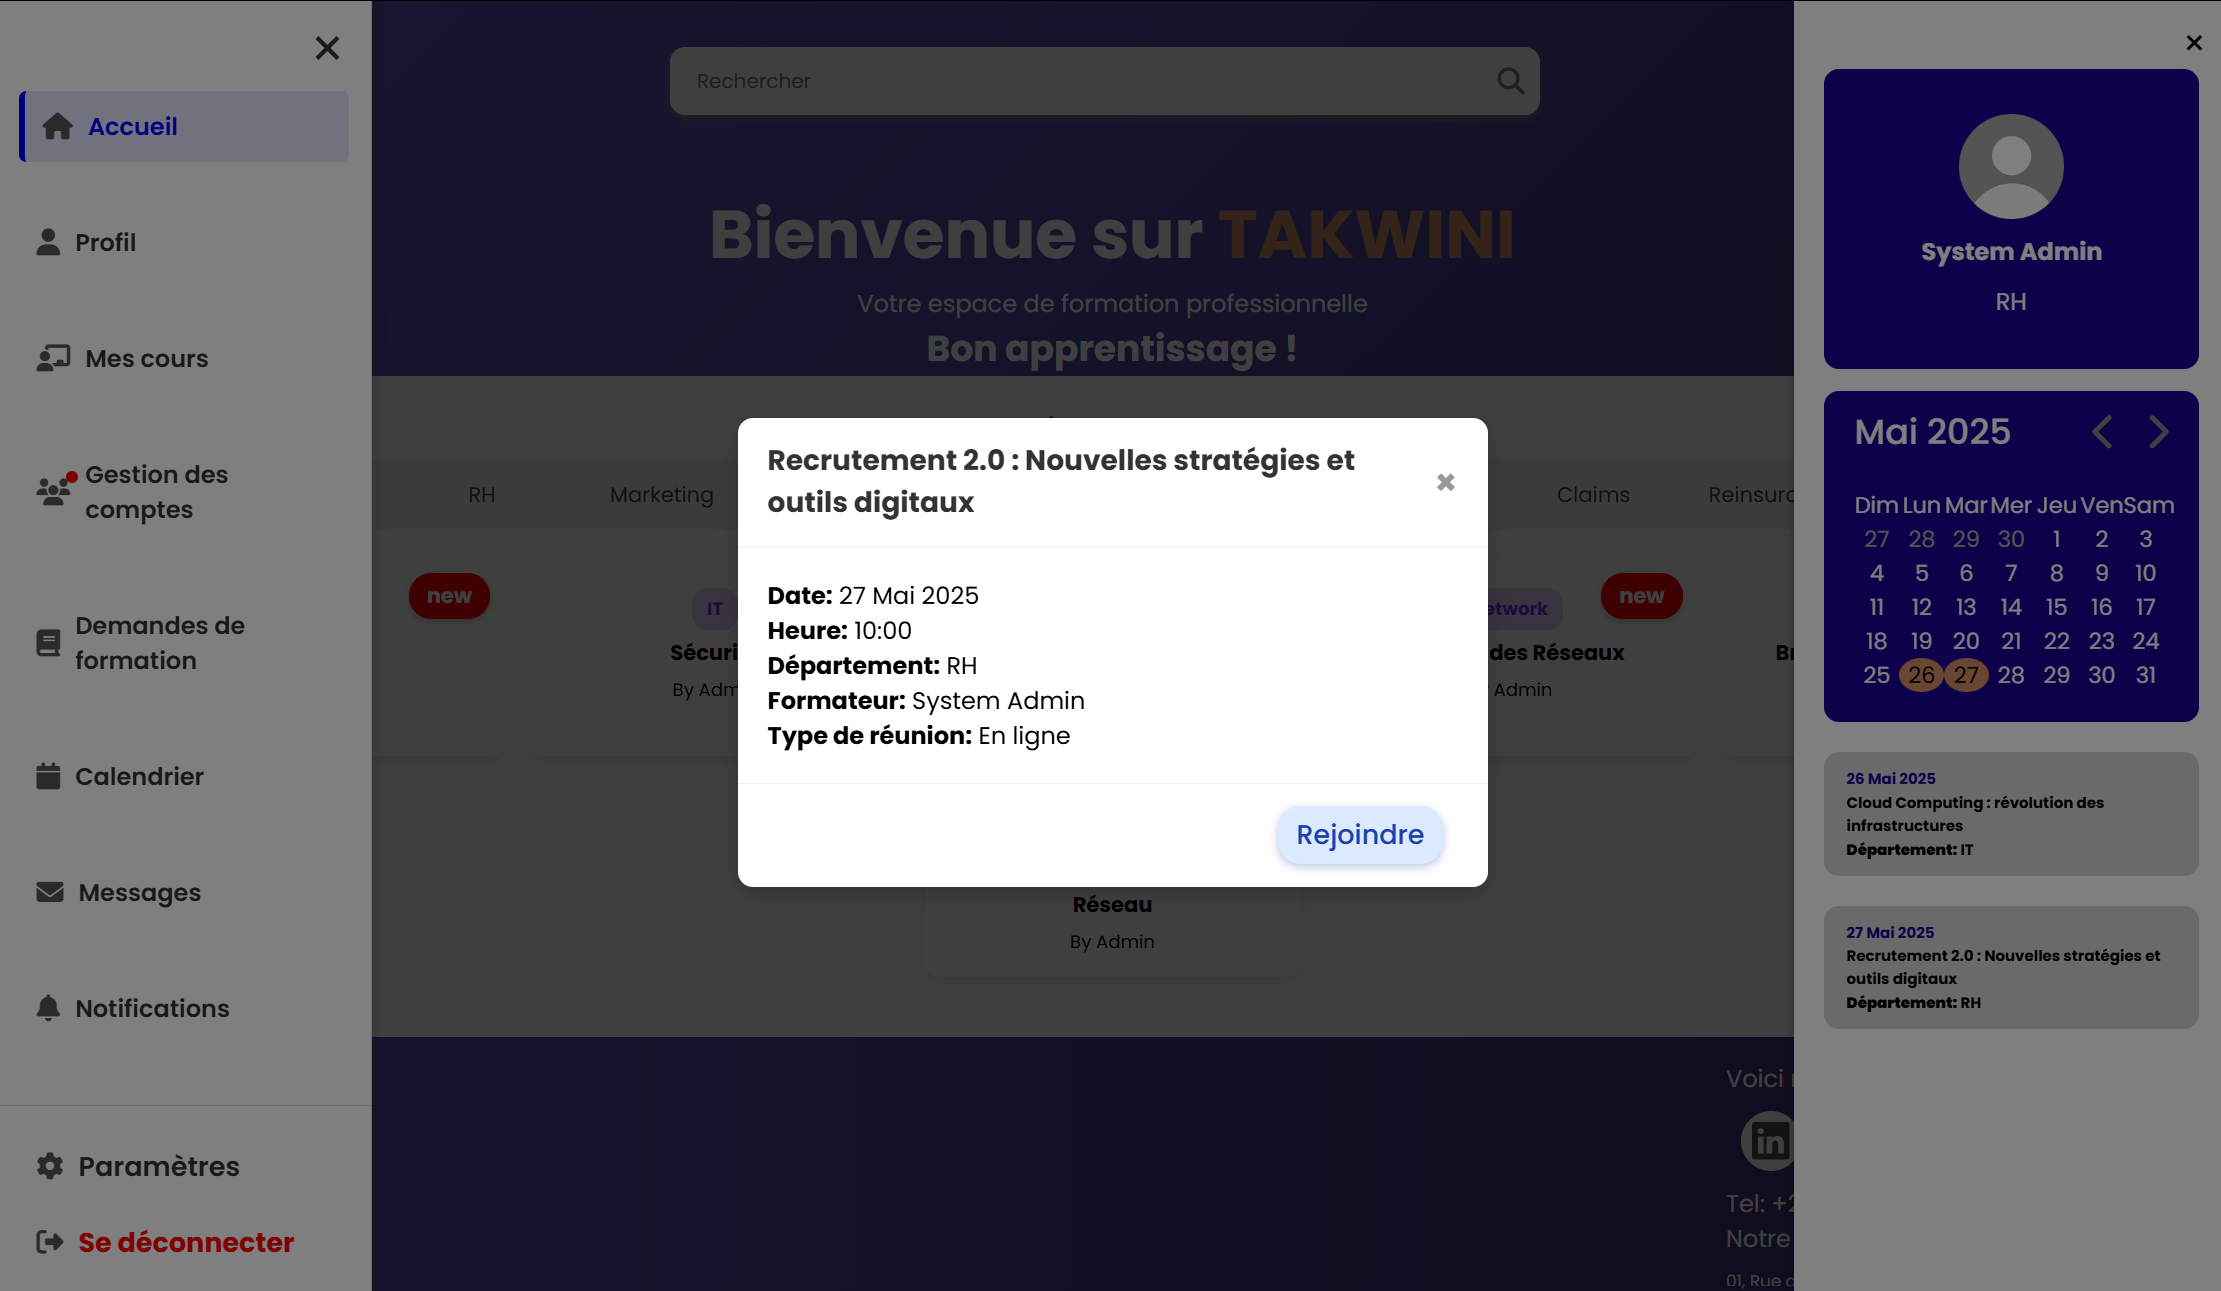
\includegraphics[width=0.6\textwidth]{coné.png}
  \caption{Barres latérales de consultation des conférences et de navigation sur la plateforme}
  \label{fig:dashboard3}
\end{figure}

\begin{figure}[H]
  \centering
  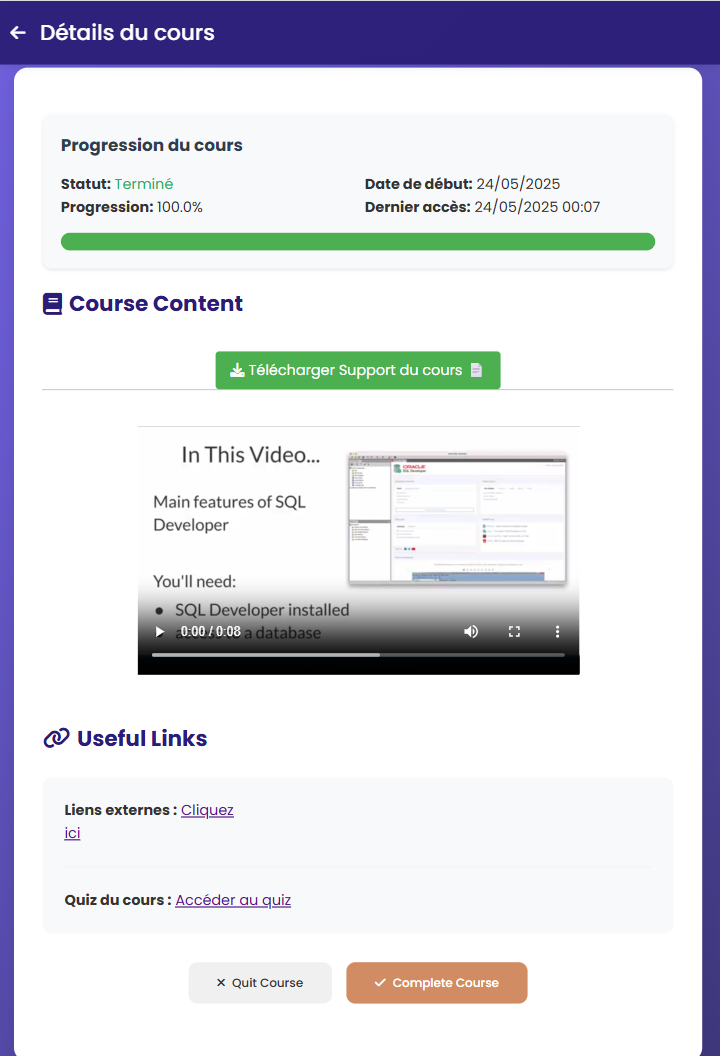
\includegraphics[width=0.6\textwidth]{courr.png}
  \caption{Interface du cours}
  \label{fig:dashboard2}
\end{figure}

\begin{figure}[H]
  \centering
  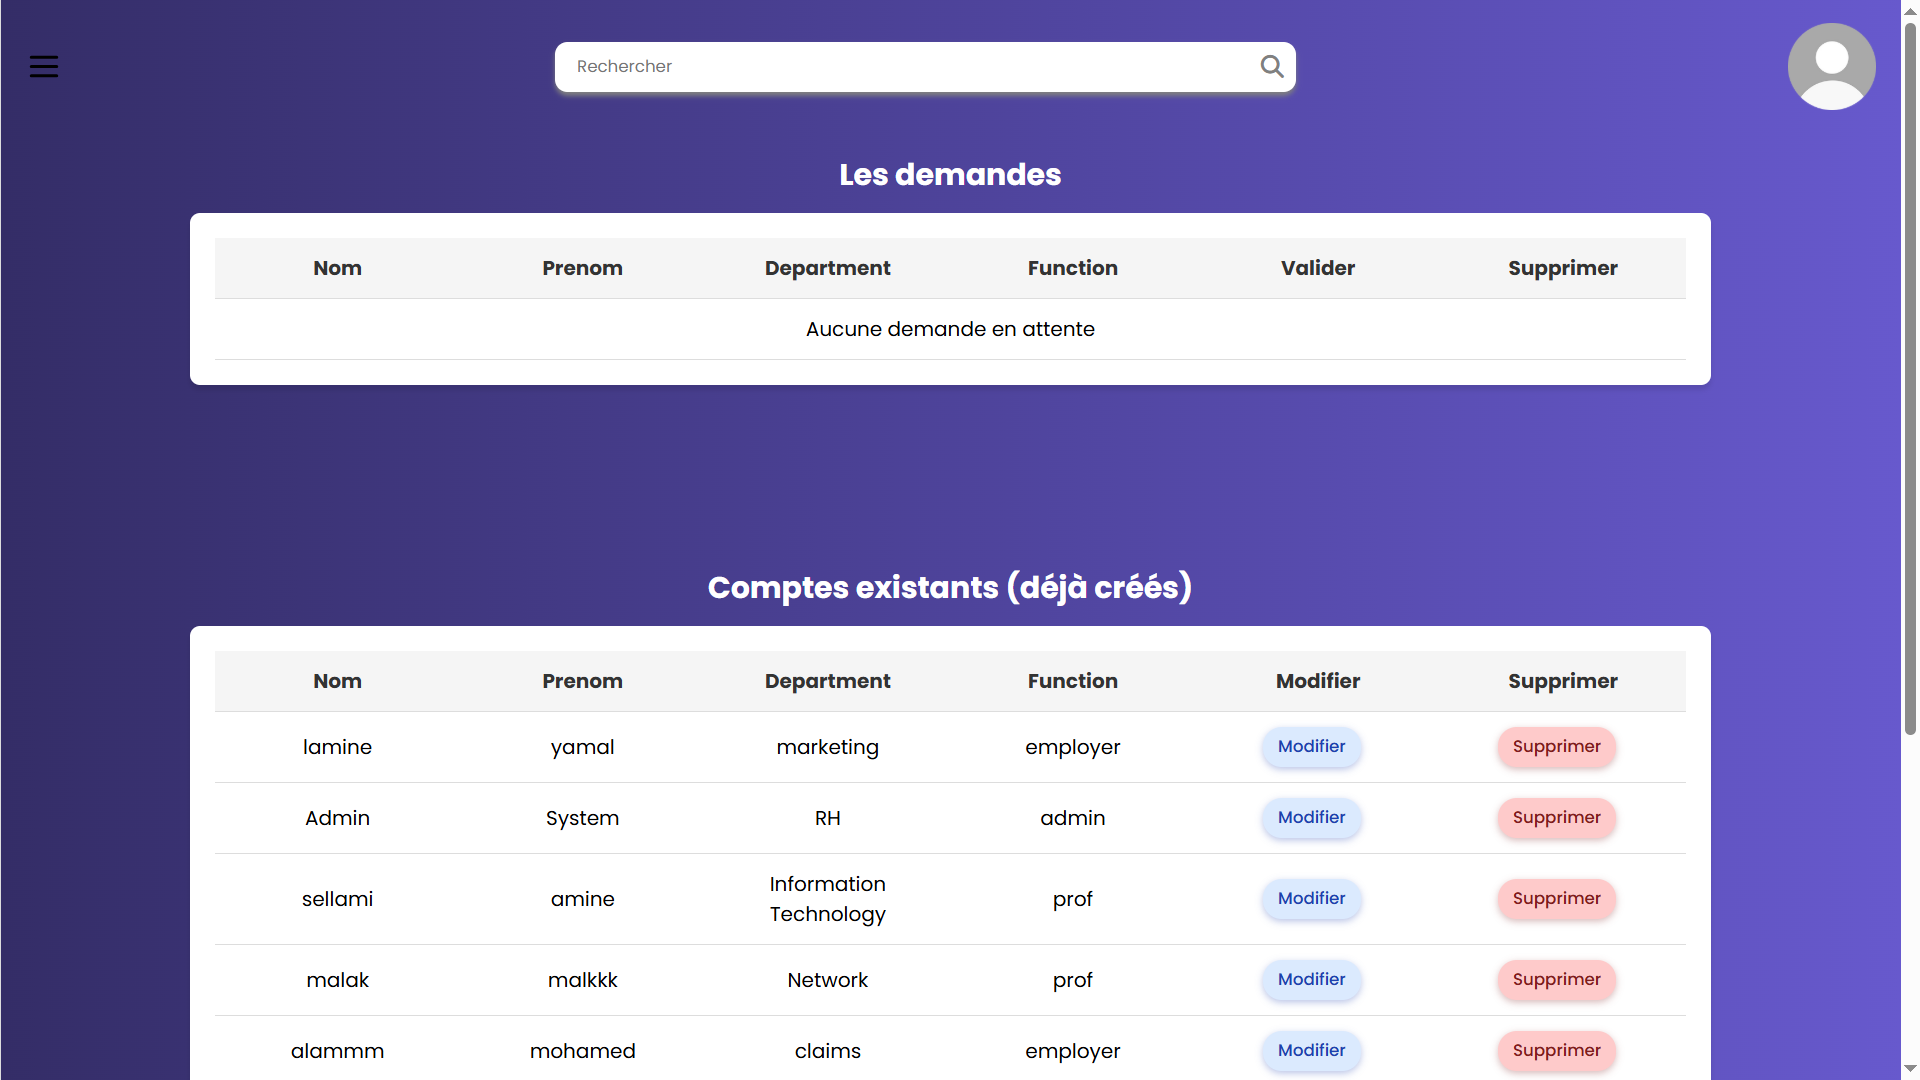
\includegraphics[width=0.6\textwidth]{compte.png}
  \caption{La gestion des comptes coté administrateur}
  \label{fig:comptr}
\end{figure}




\begin{figure}[H]
  \centering
  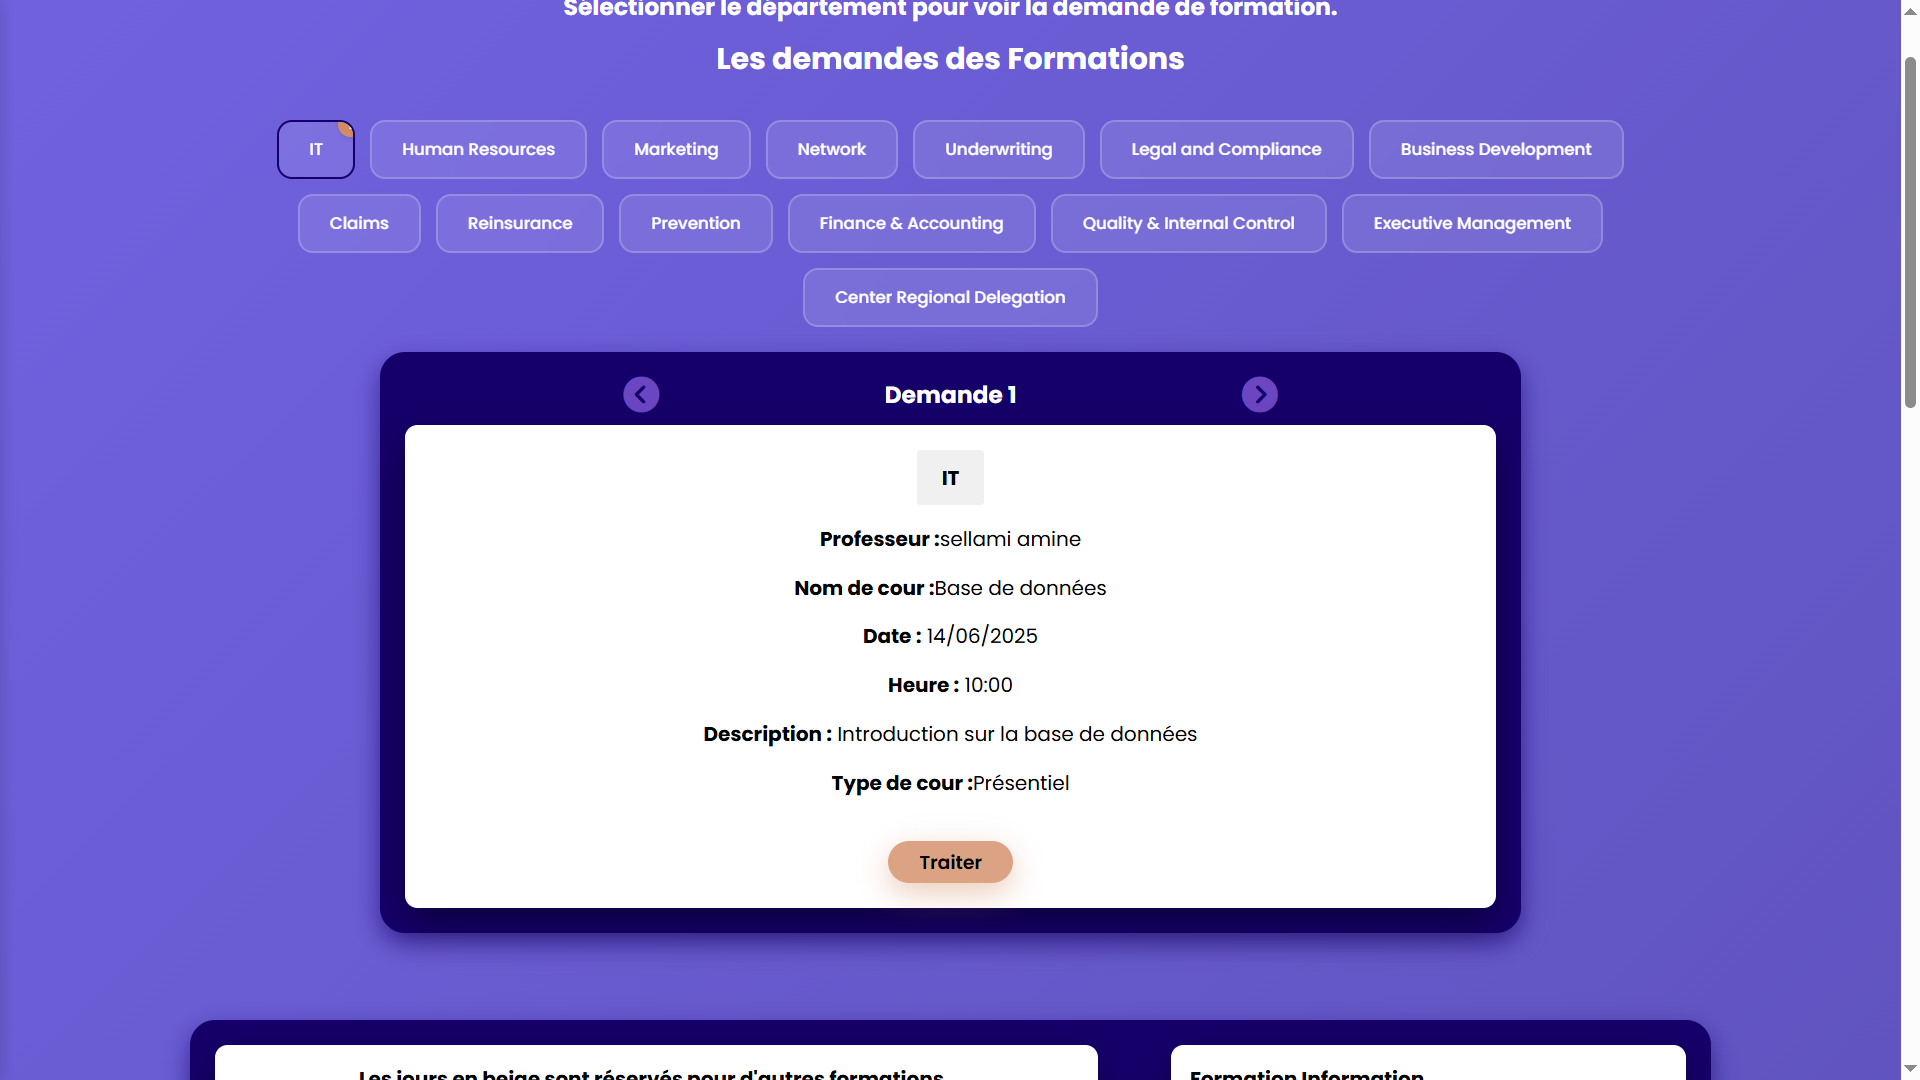
\includegraphics[width=0.6\textwidth]{dem.png}
  \caption{L'interface pour traiter les demandes de conférence "administrateur"}
  \label{fig:traitment}
\end{figure}

\begin{figure}[H]
  \centering
  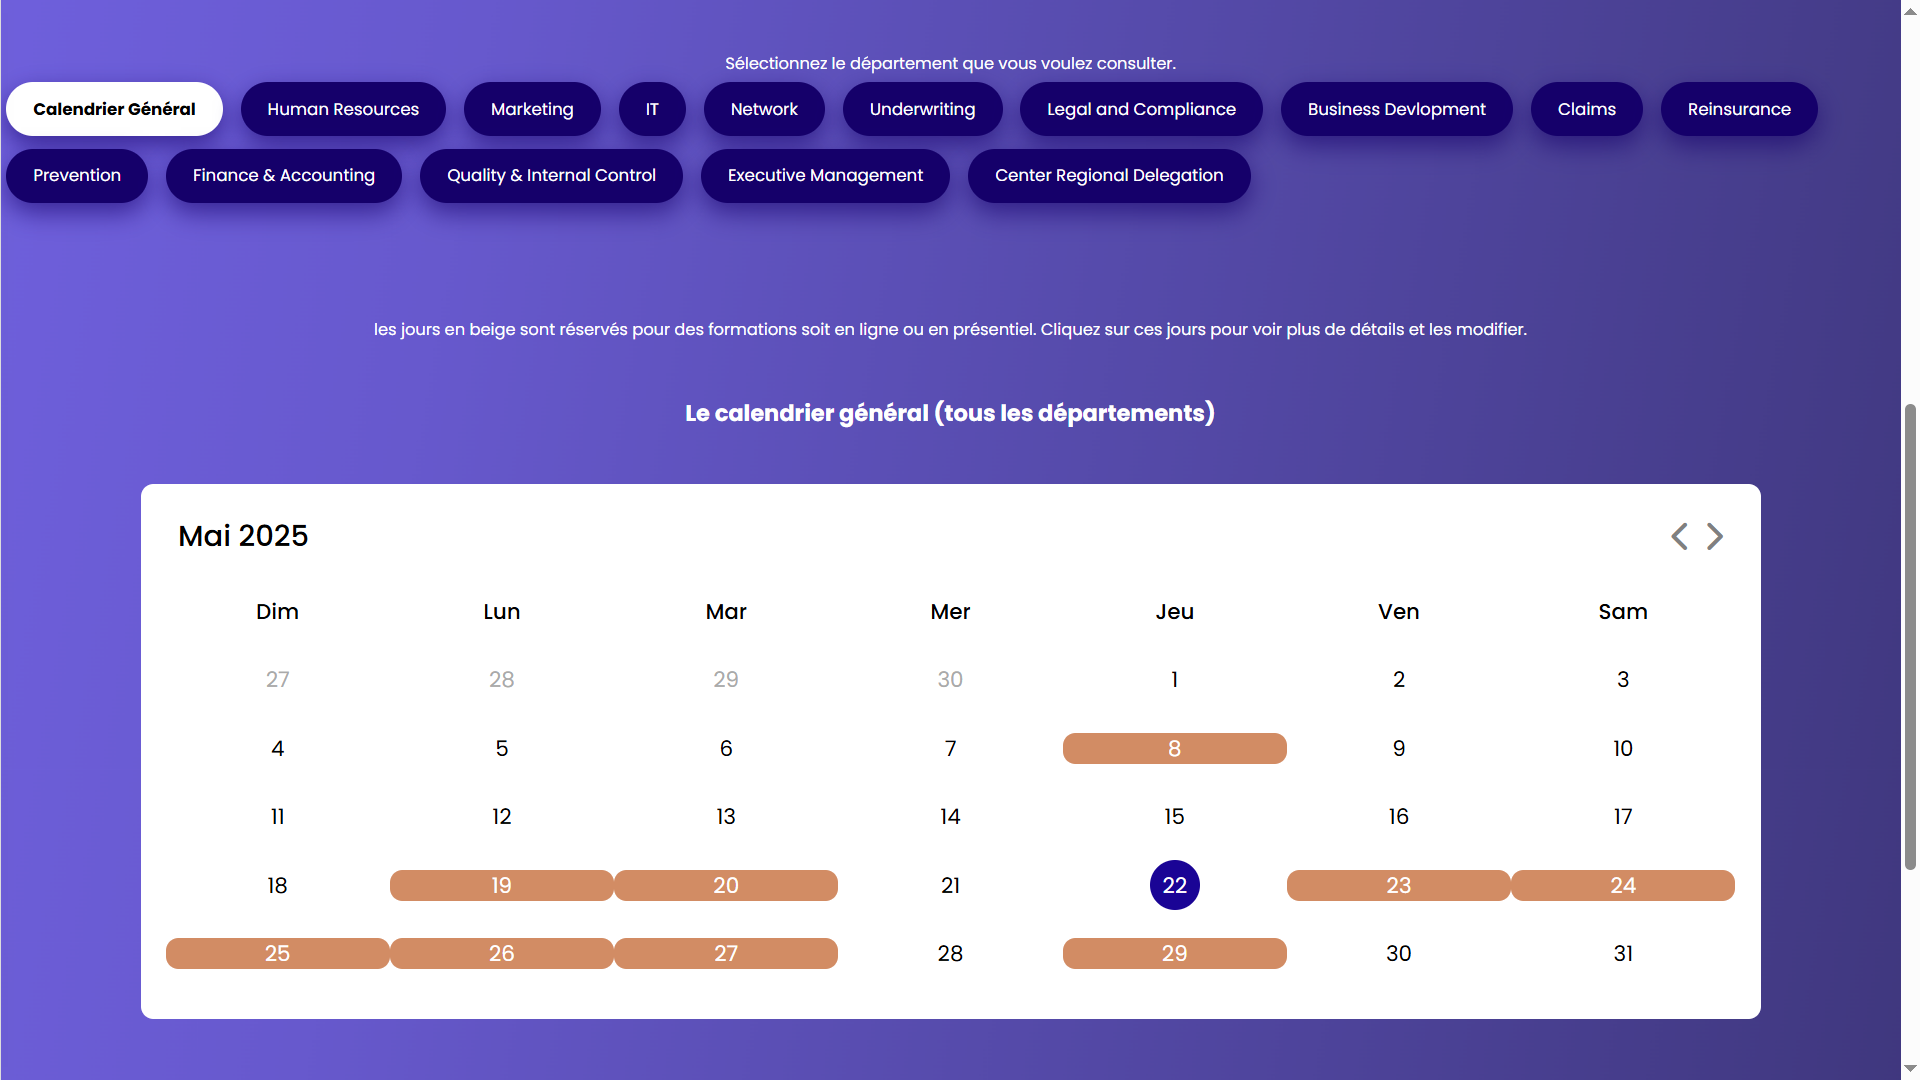
\includegraphics[width=0.6\textwidth]{modconsfor.png}
  \caption{L'interface pour consulter et modifier les conférences "administrateur"}
  \label{fig:modsup}
\end{figure}




\begin{figure}[H]
  \centering
  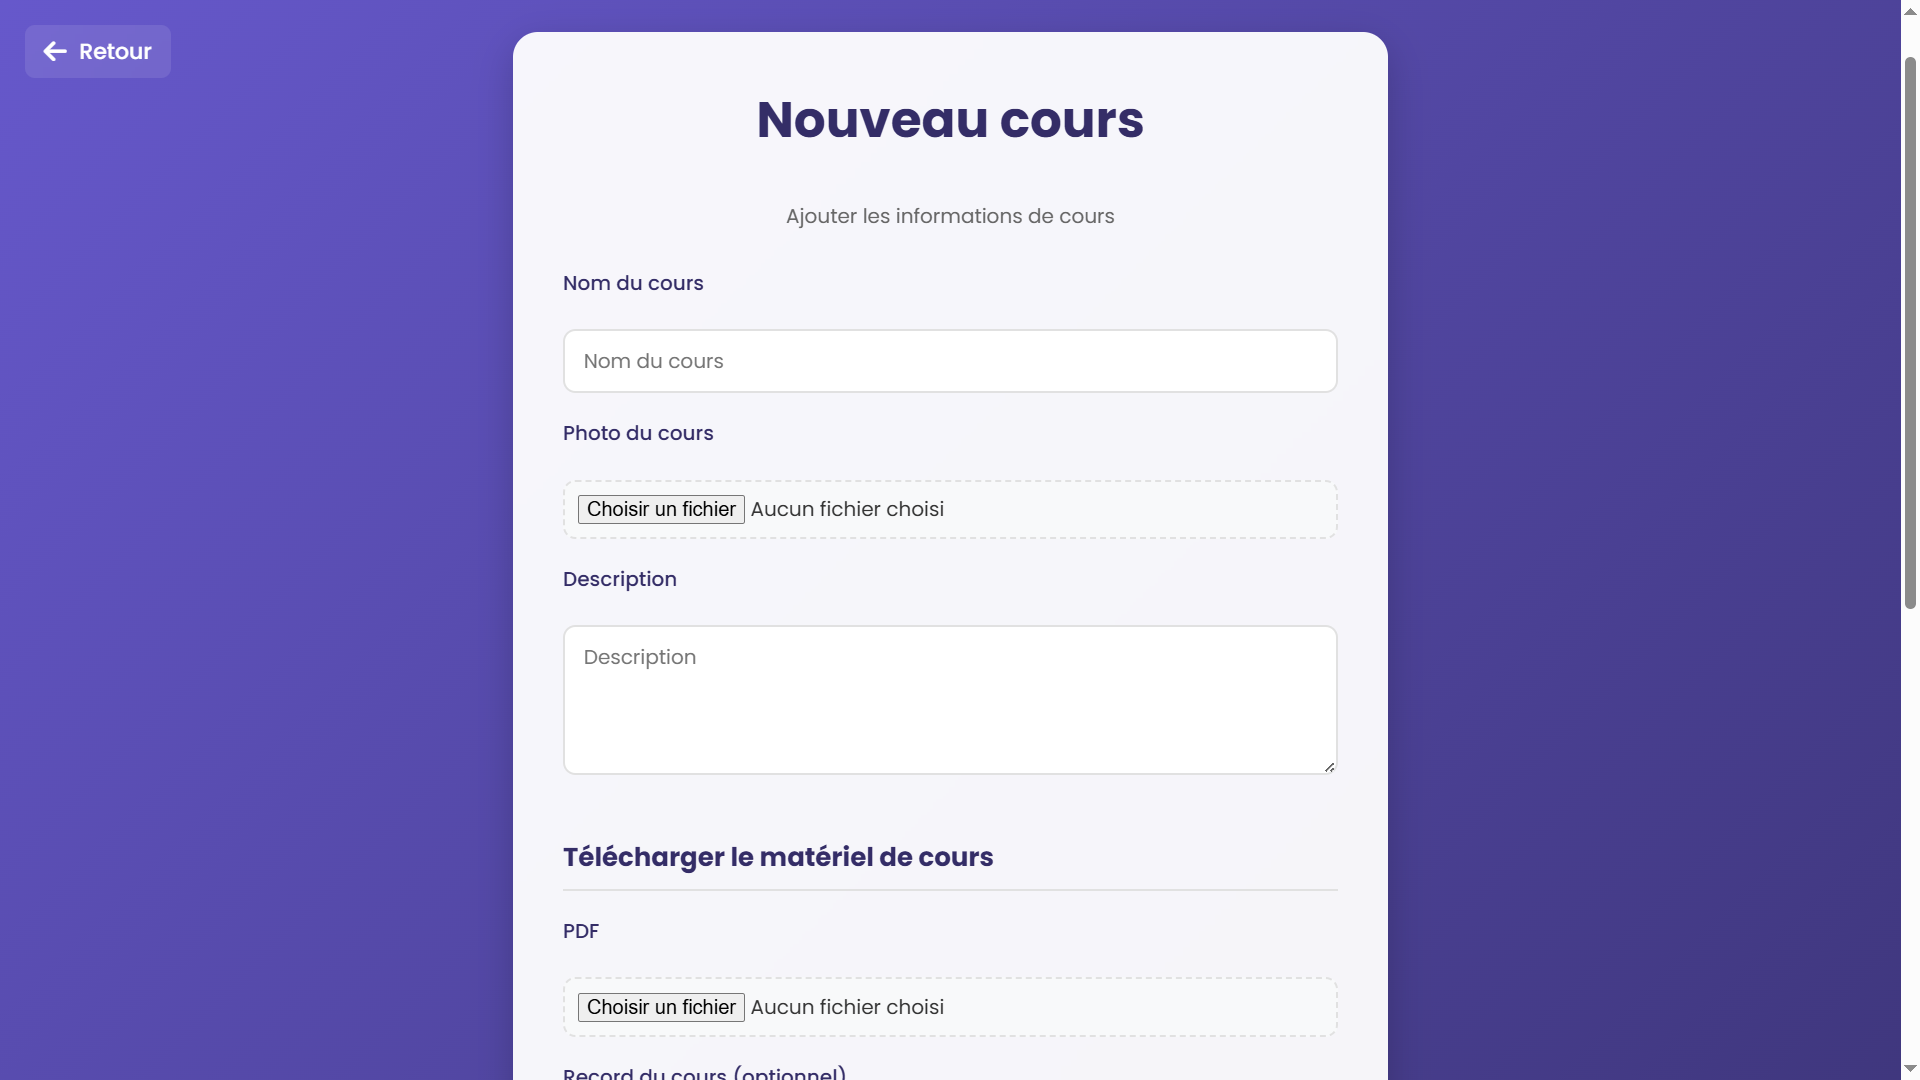
\includegraphics[width=0.6\textwidth]{creacou.png}
  \caption{L'interface pour ajouter des ressources pédagogique "professeur et administrateur"}
  \label{fig:ressource}
\end{figure}


\begin{figure}[H]
  \centering
  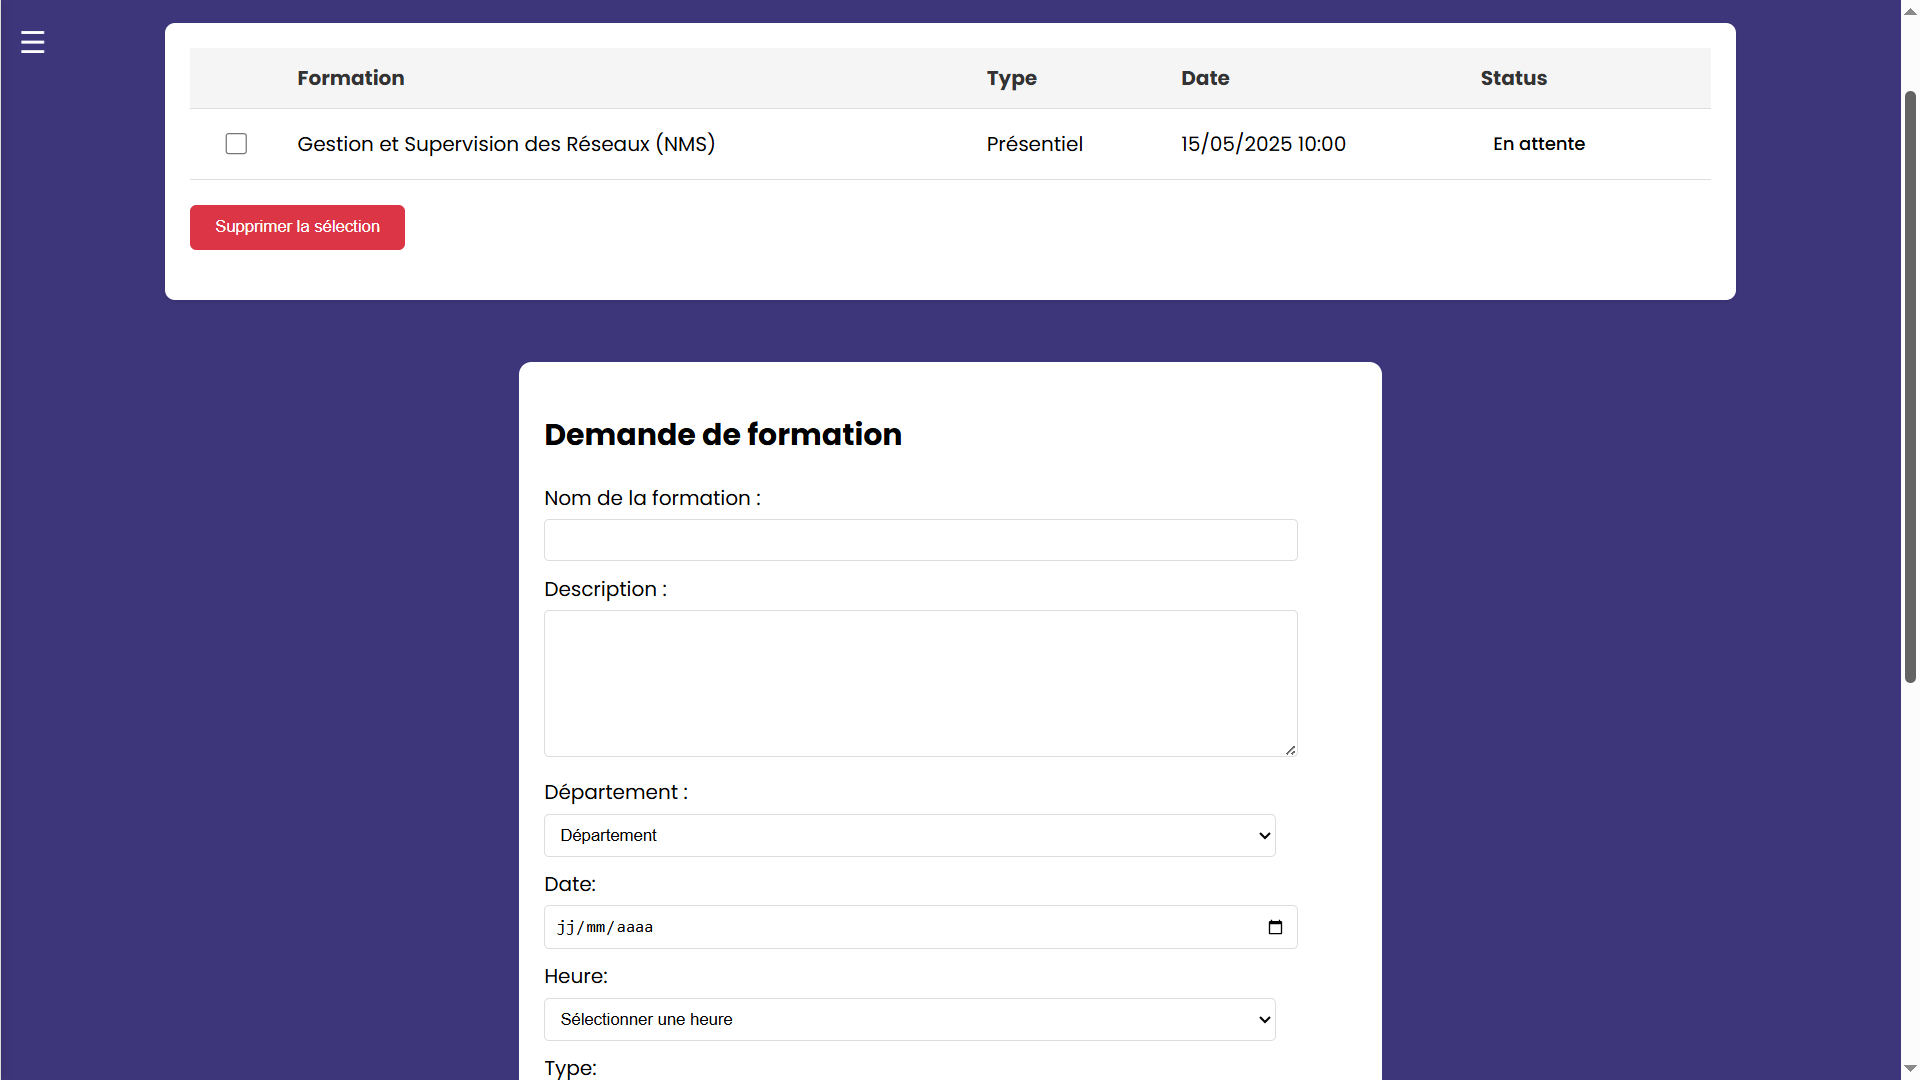
\includegraphics[width=0.6\textwidth]{planiconf.png}
  \caption{L'interface pour envoyer la demande et la consultaion d'état de conférence "professeur"}
  \label{fig:planif}
\end{figure}

\begin{figure}[H]
  \centering
  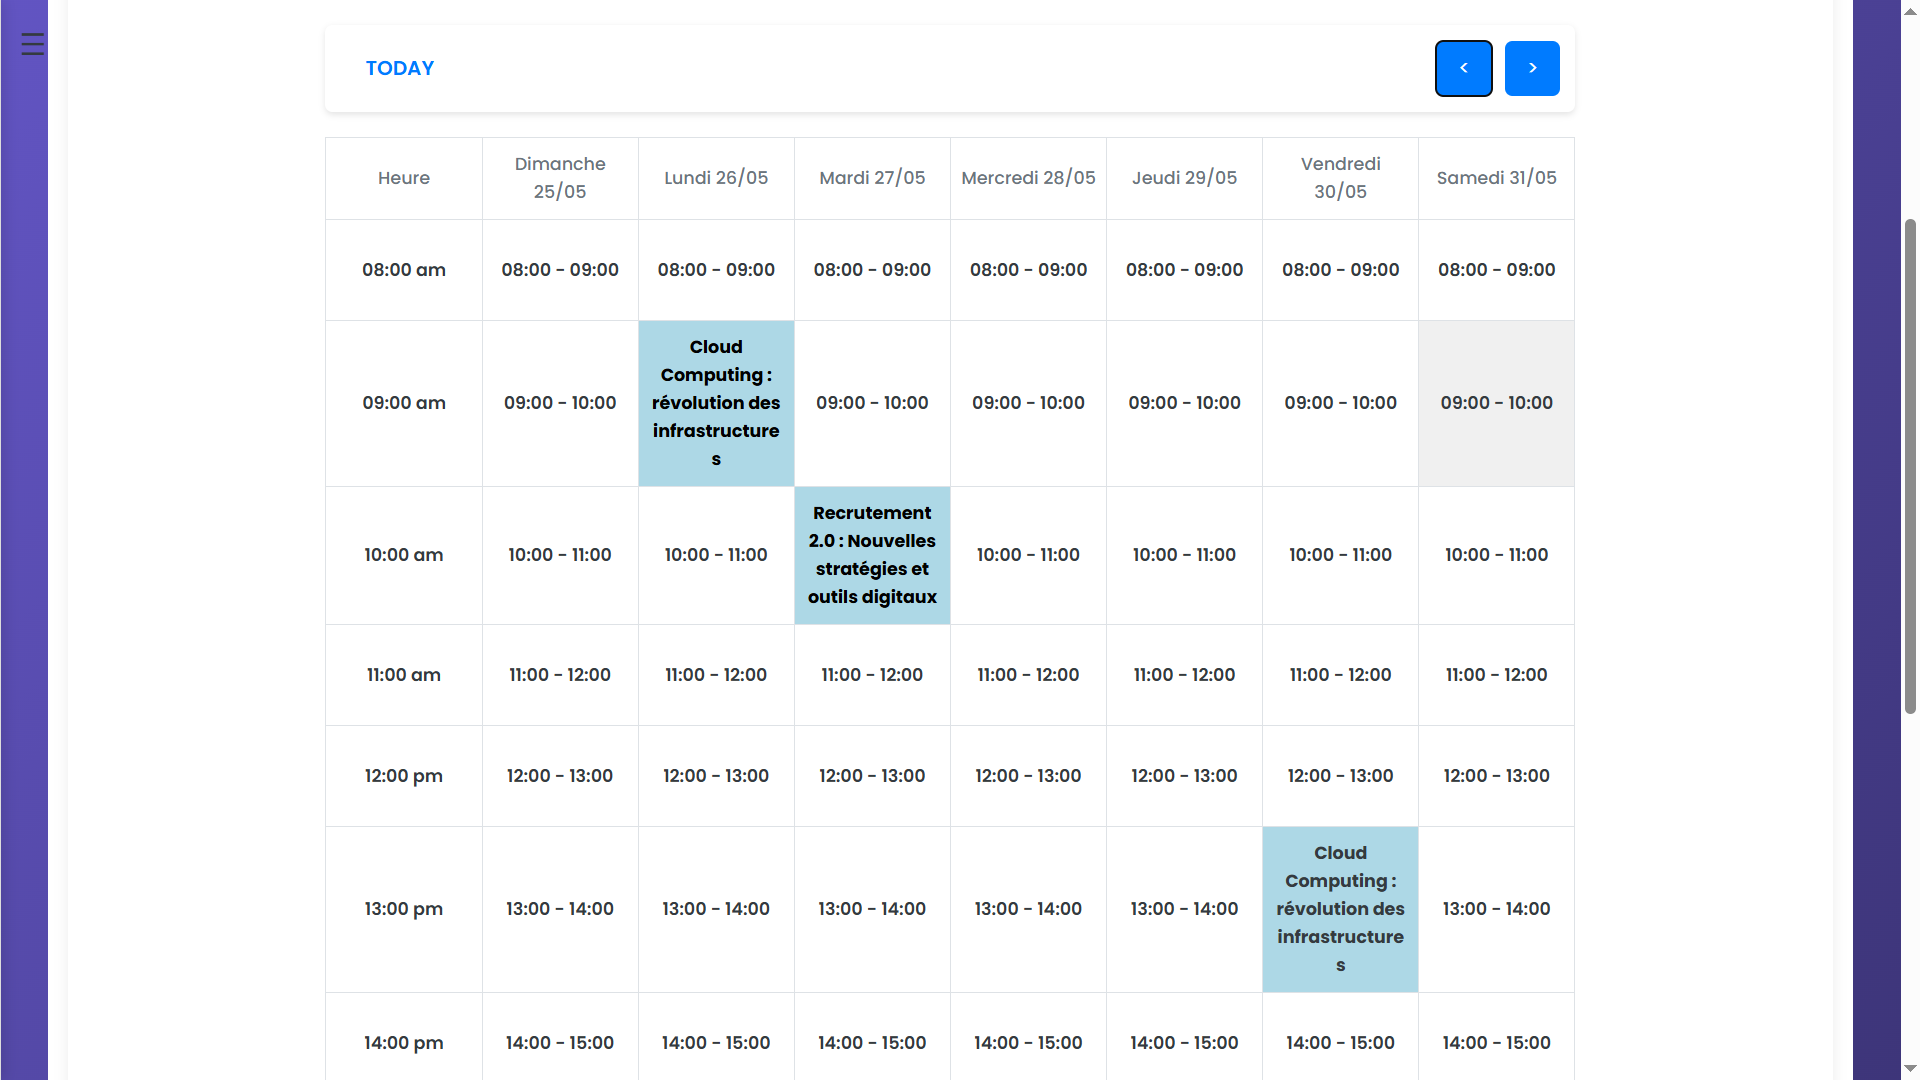
\includegraphics[width=0.6\textwidth]{calendarprof.png}
  \caption{Calendrier associé au professeur}
  \label{fig:planif1}
\end{figure}

\begin{figure}[H]
  \centering
  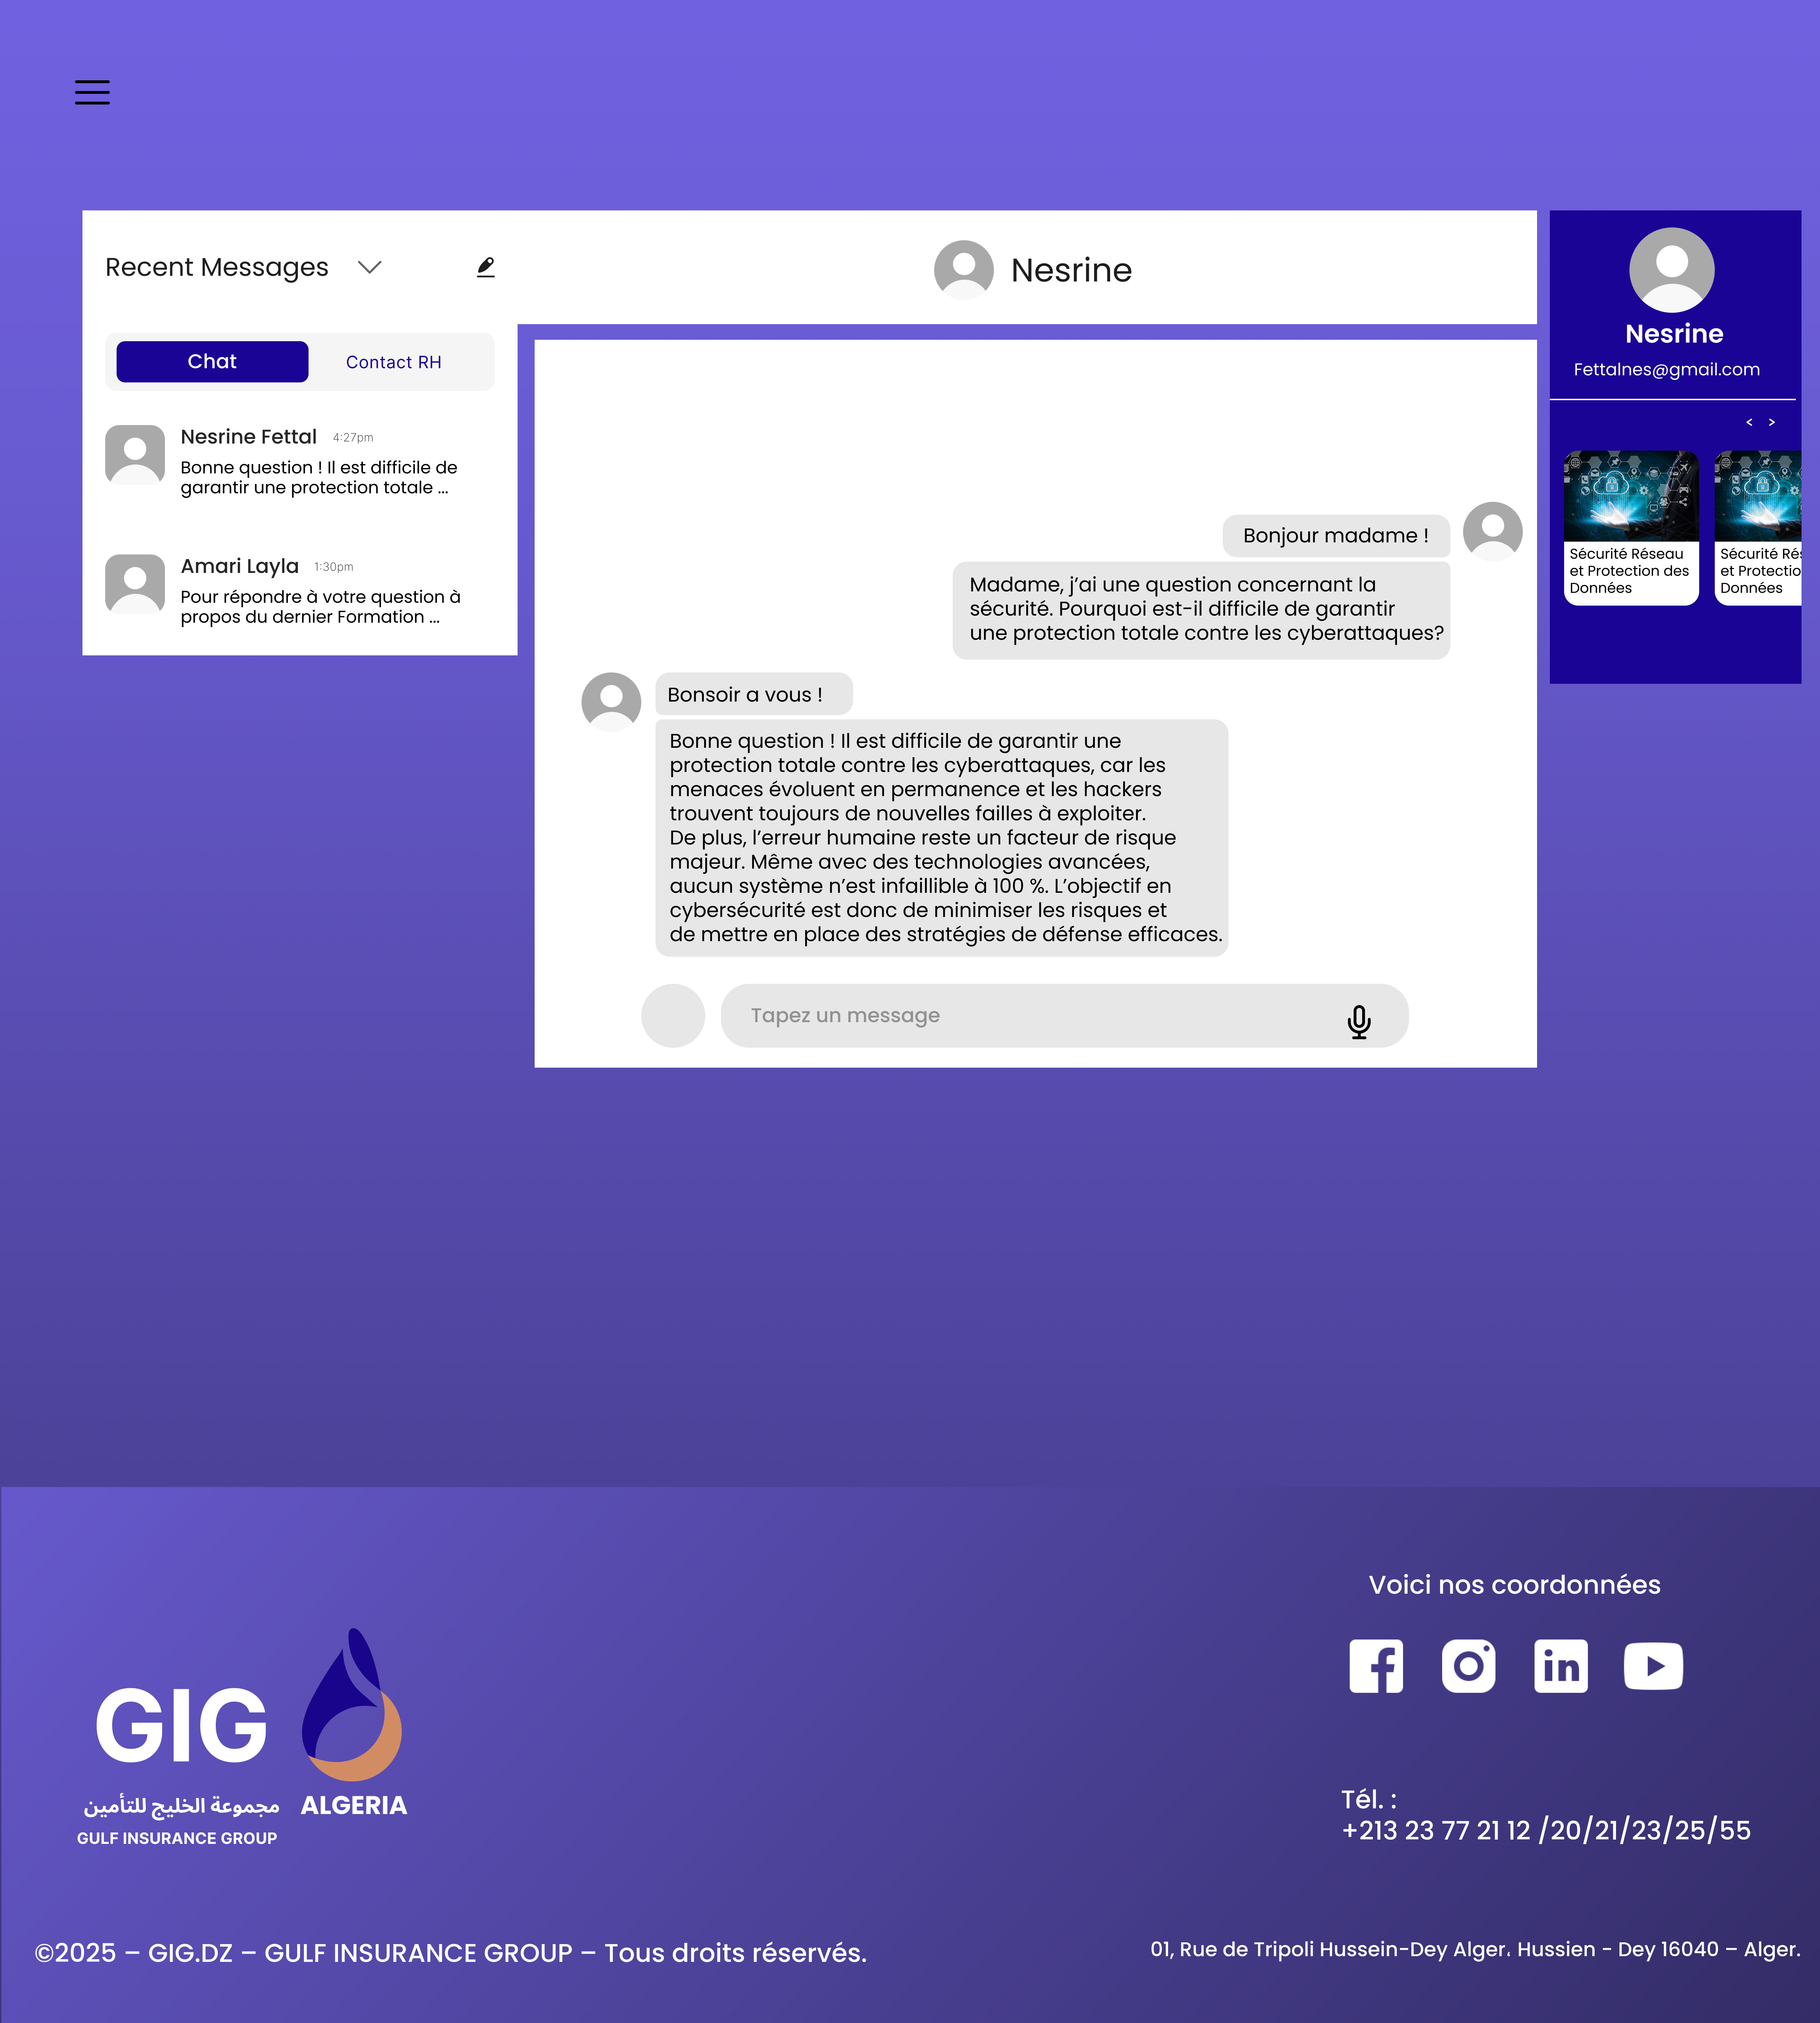
\includegraphics[width=0.6\textwidth]{messages.png}
  \caption{Interface de messagerie pour assurer la communication entre utilisateurs}
  \label{fig:planif2}
\end{figure}


La plateforme TAKWINI est responsive et s’adapte à tous les types d’écrans, que ce soit des ordinateurs ou des téléphones. 




\begin{figure}[H]
  \centering
  \begin{subfigure}[t]{0.4\textwidth}
    \centering
    
\includegraphics[width=\textwidth]{courtlphn.jpg}
    \caption{Interface d’accueil sur smartphone }
    \label{fig:courtlphn}
  \end{subfigure}
    \hspace{1cm}
    \begin{subfigure}[t]{0.4\textwidth}
      \centering
      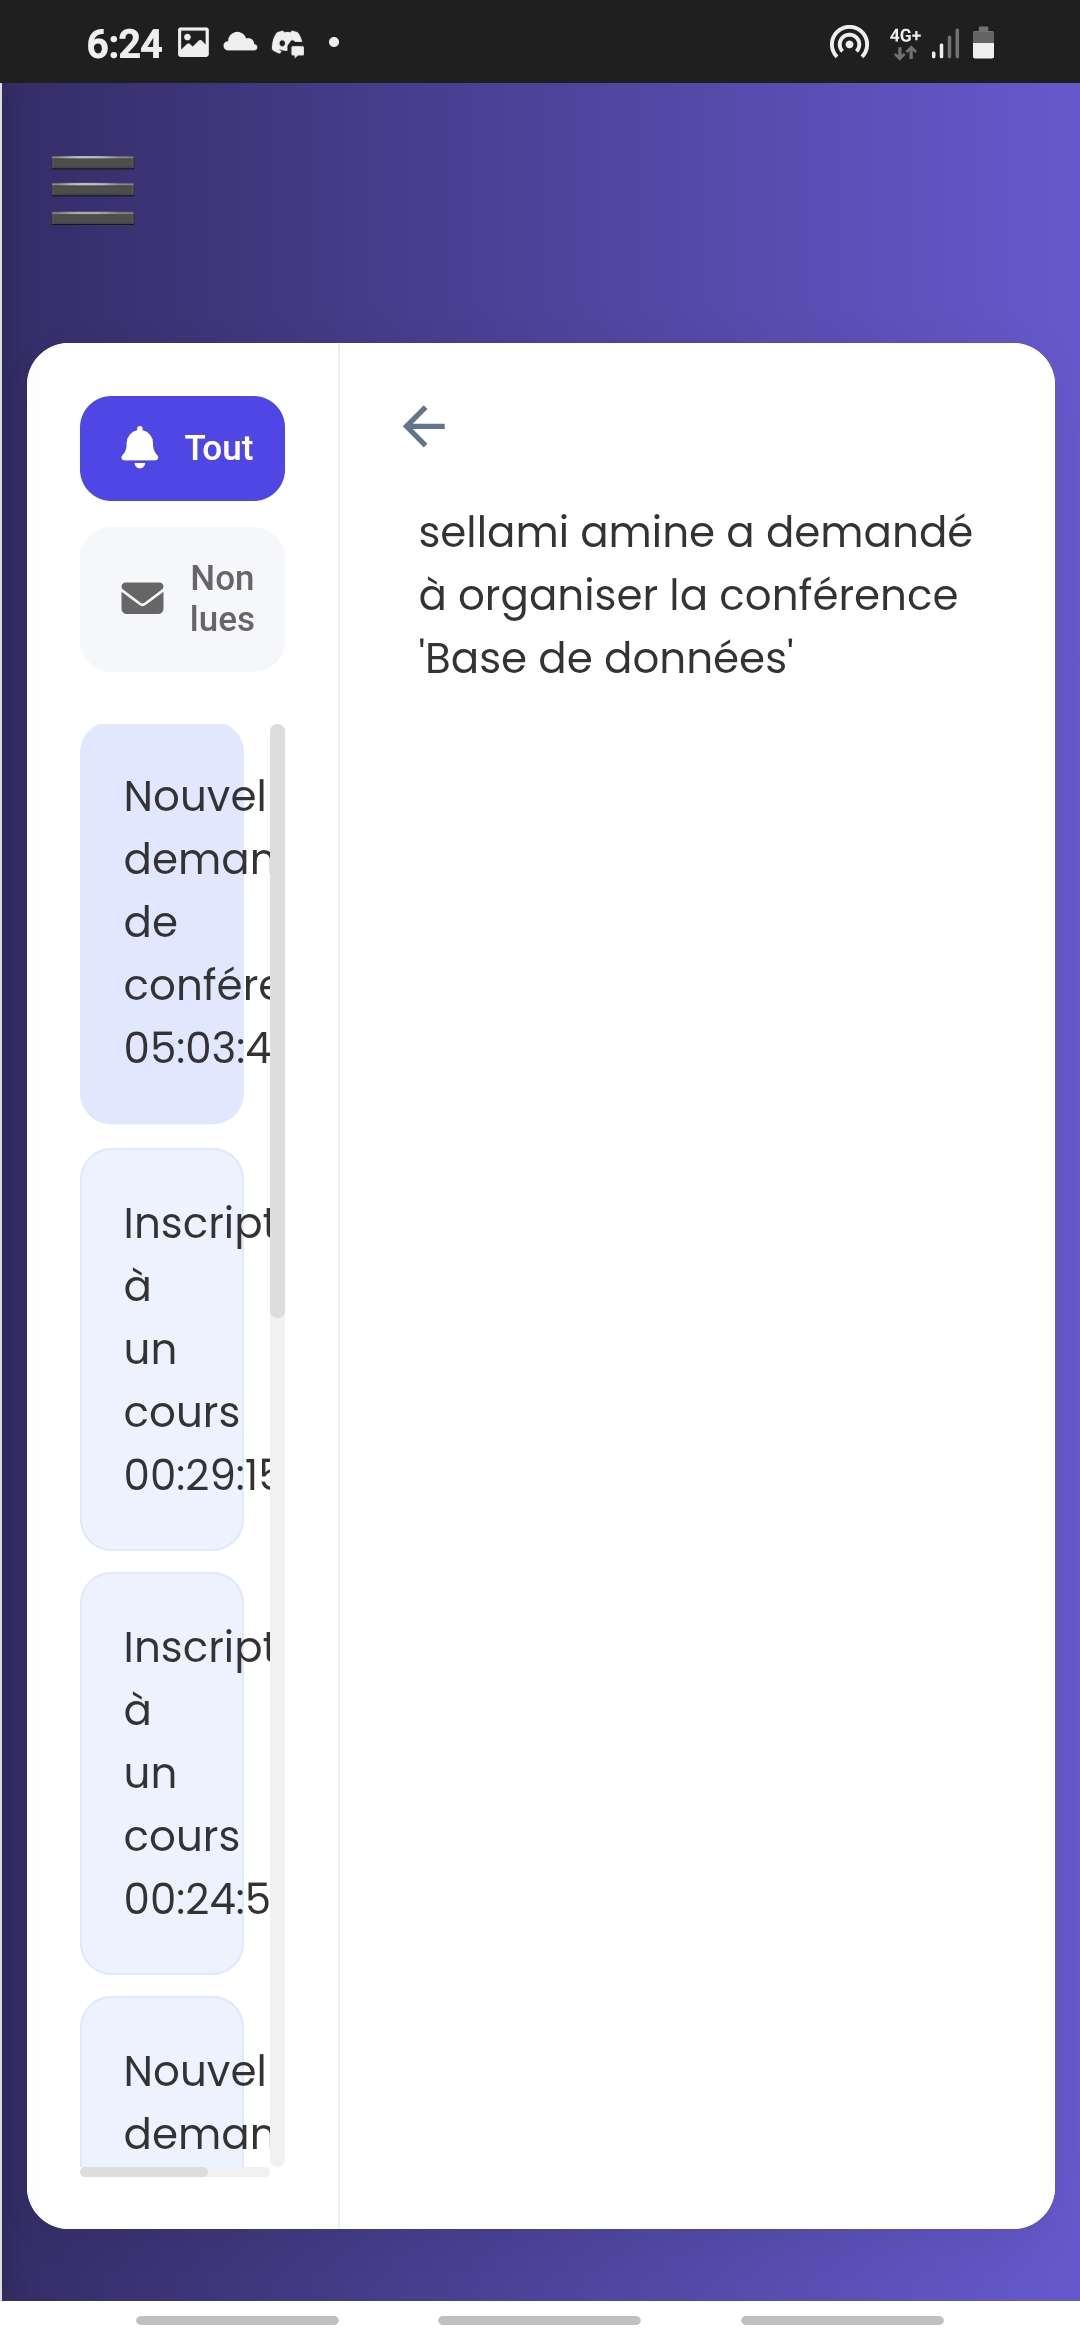
\includegraphics[width=\textwidth]{notif.jpg}
      \caption{Interface des notifications}
      \label{fig:notif}
  \end{subfigure}
  \label{fig:login}
\end{figure}




\newpage
\section{Conclusion}
\begin{spacing}{1,3}
    


\vspace{0,5cm}

Cette étude a été réalisée dans le but d’analyser tous les avantages et les inconvénients des solutions adaptables par Gulf Insurance Group Algeria, ainsi que d’évaluer les solutions déjà existantes sur le marché et d’expliquer pourquoi elles ne constituent pas une solution parfaitement adaptée aux besoins spécifiques de l’entreprise.

\vspace{1cm}


Notre objectif principal était d’offrir à l’entreprise un contrôle total sur la gestion de ses formations, en assurant une indépendance vis-à-vis des solutions externes, afin d’éviter les inconvénients potentiels liés à leur utilisation. Ce choix permet également de réduire les coûts inutiles.

\vspace{1cm}


Dans ce cadre, nous avons conçu la plateforme TAKWINI pour faciliter l’apprentissage et améliorer les compétences des employés de manière fluide et accessible à tous les utilisateurs. La plateforme leur permet de consulter, à tout moment, les contenus pédagogiques et les conférences, selon leurs besoins. Elle offre aussi aux professeurs et au service des ressources humaines un outil pour planifier efficacement les conférences. La plateforme a été sécurisée et entièrement personnalisée pour qu’elle soit accessible uniquement aux personnes autorisées.




\vspace{1cm}



TAKWINI satisfait bien les exigences actuelles de Gulf Insurance Group Algeria, mais il reste plusieurs domaines où des améliorations sont possibles. Pour l'avenir, nous envisageons d'ajouter un espace consacré au suivi des conférences en ligne directement sur la plateforme, ainsi qu'un système de tests de niveau interne afin d’optimiser le suivi de la progression des employés. Nous avons également l'intention d'implémenter des fonctions basées sur l'intelligence artificielle, notamment pour la création automatique de quiz, qui permettra d’évaluer la compréhension des apprenants.
\end{spacing}


\newpage
\section{Annexe}
\appendix
\section{Le diagramme d'authentification}
\label{annexe-auth}

\begin{figure}[H]
  \centering
  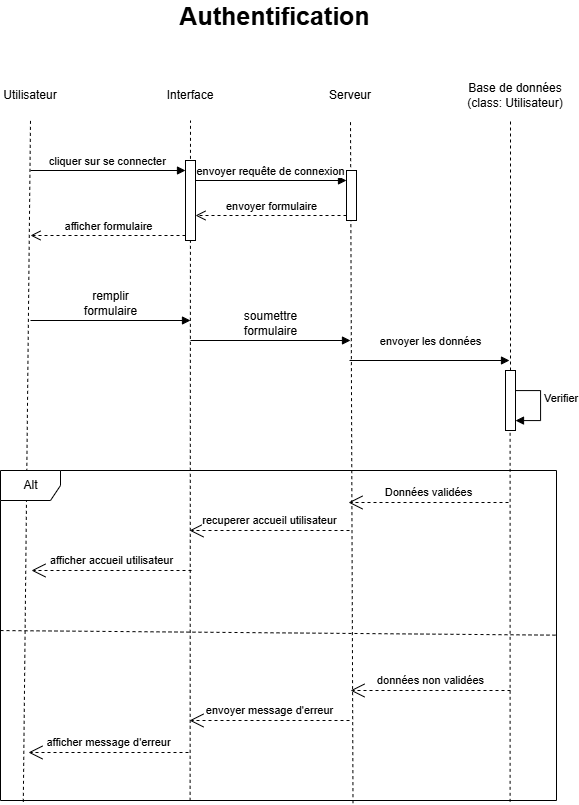
\includegraphics[width=0.6\textwidth]{authentification(1.2).drawio.png}
  \caption{Diagramme de Séquence pour l'authentification}
  \end{figure}


\section{Le reste du design de la plateforme TAKWINI}
\label{annexe-design}

\begin{figure}[H]
  \centering
  
\includegraphics[width=0.6\textwidth]{homee.png}
  \caption{Design de l'interface avec Figma}
  \end{figure}

  
\begin{figure}[H]
  \centering
  \includegraphics[width=0.6\textwidth]{Dashboard RH.png}
  \caption{Design de l'accueil de professeur et administrateur}
  \end{figure}

  
\begin{figure}[H]
  \centering
  
\includegraphics[width=0.6\textwidth]{Ajoute-formation.png}
  \caption{Design de calendrier pour supprimer et modifier les conférences}
  \end{figure}










\section{Définition de l'architecture client-serveur }
En informatique, l'architecture client-serveur est un modèle de réseau où un client demande des services ou des ressources à un serveur. Le frontend est la partie visible d'une application avec laquelle l'utilisateur interagit, tandis que le backend gère la logique, les données et les processus en arrière-plan. 
Architecture client-serveur :
Client :
C'est l'ordinateur ou l'application qui demande des services ou des ressources à un serveur. 
Serveur :
Un ordinateur ou une application qui héberge, fournit et gère les ressources et les services destinés aux clients. 
\label{annexe-client-ser}


\newpage
\begin{center}
{\Huge \textbf{\textit{Bibliographie}}}
\vspace{1cm}
% \printbibliography
\printbibliography[heading=none]





\end{center}
\end{document}
